\documentclass[a4paper,landscape]{article}
\usepackage[utf8]{inputenc}
\usepackage{graphicx}
\usepackage{float}
\usepackage{geometry}
\geometry{margin=1in}
\usepackage{caption}
\usepackage{hyperref}
\usepackage{xcolor}

\title{Data Visualization Portfolio}
\author{Alan Copa}
\date{Data Analytics for Finance I \& II, 2024-2025}

\begin{document}
\maketitle
\begin{figure}[H]
    \centering
    \includegraphics[width=0.31\textwidth]{Visualizations/DALL·E 2025-01-13.pdf}
\end{figure}

\tableofcontents


\section{Introduction}
This portfolio presents a collection of data visualizations created as part of the course Data Analytics for Finance I \& II for the 2024-2025 academic year.

\section{Visualization Tasks}

\subsection{Task 1: Bad/Manipulative Visualization}
\begin{figure}[H]
    \centering
    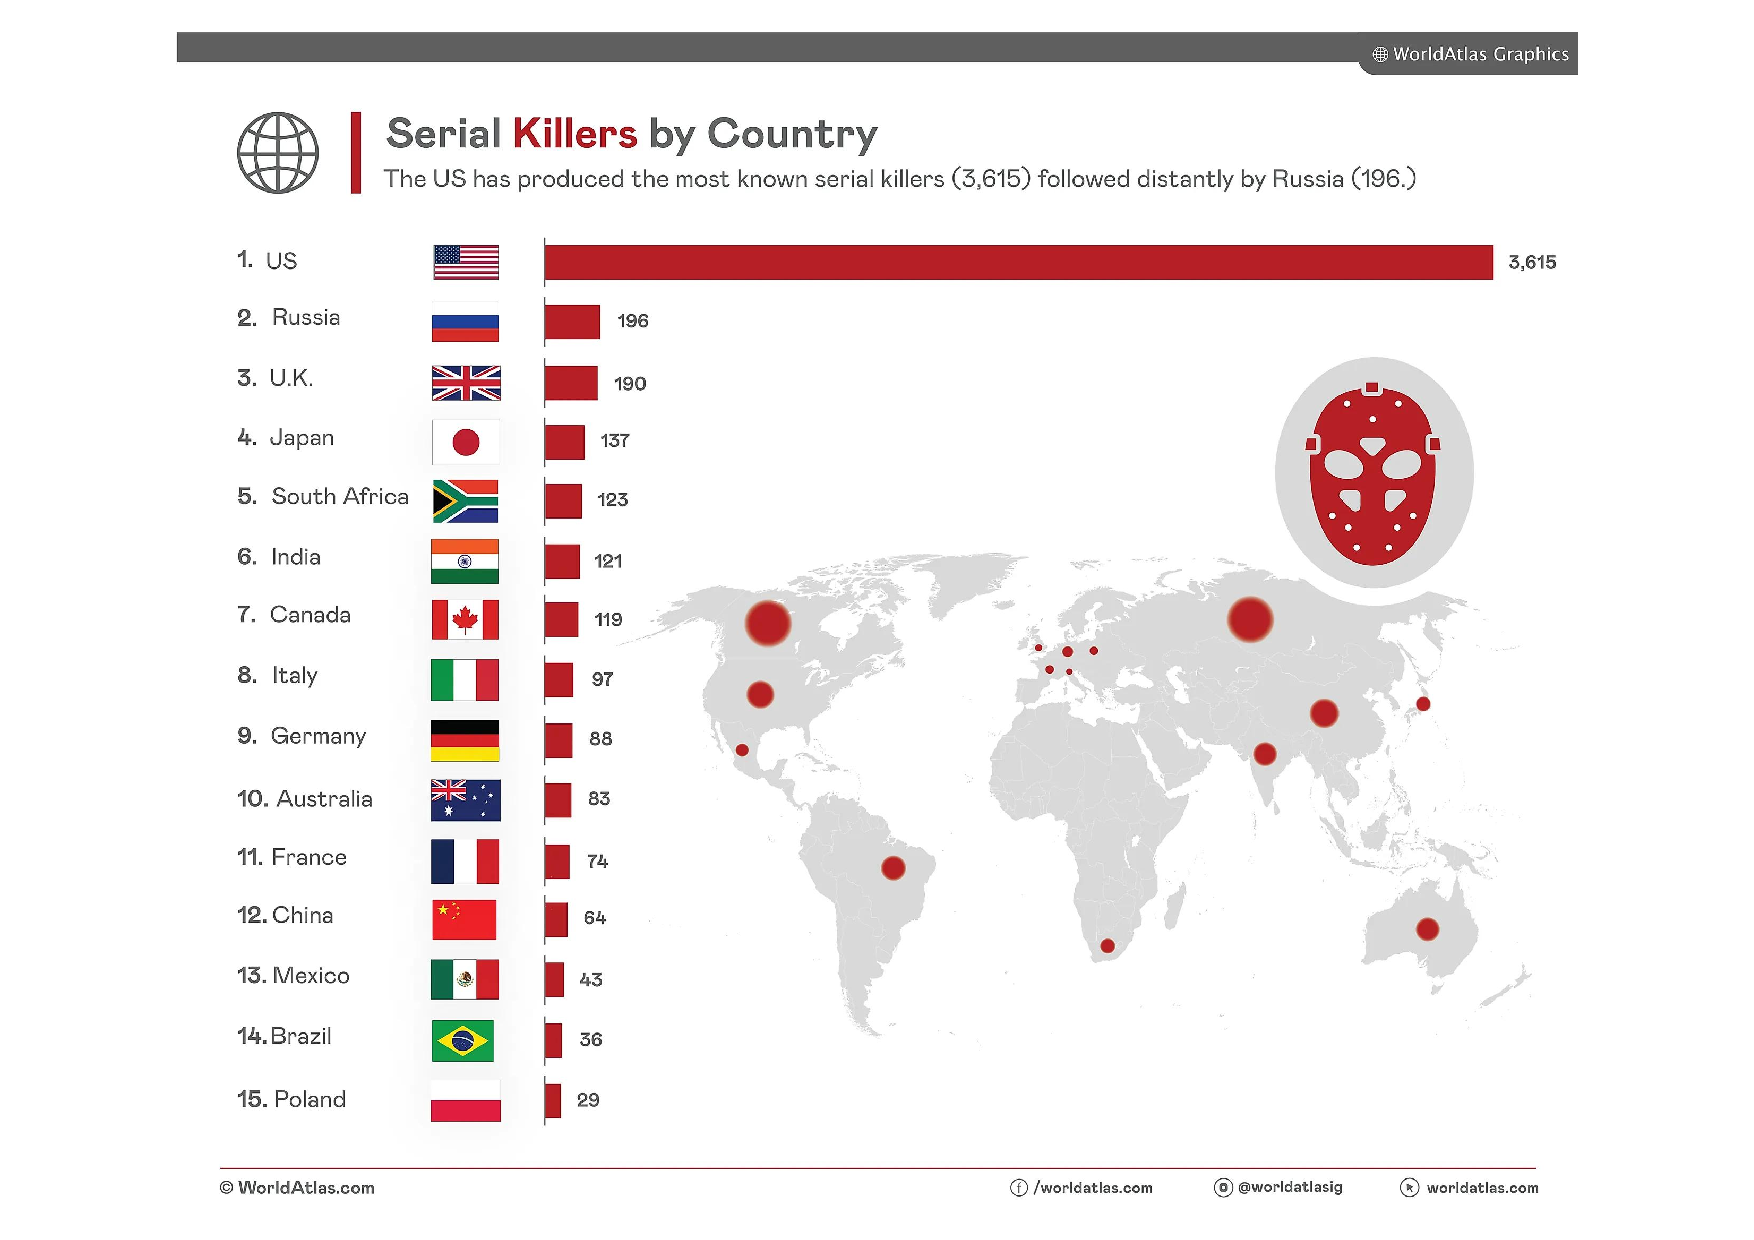
\includegraphics[width=0.6\textwidth]{Visualizations/bad-data.pdf} % Replace with your file name
    \caption{Bad Visualization \cite{worldatlas2025serialkillers}}
    \label{fig:bad}
\end{figure}

\subsubsection{Critique}
This data visualization is misleading because the values in the horizontal bar chart are presented as the absolute number of serial killers per country. The proportion relative to the population of each country is not considered, resulting in an overwhelming scale for the US, which overshadows the other values. The addition of the map without a proper legend adds confusion, as the red circles are not proportional to the data shown. This suggests an alternative perspective but fails to clarify it. Consequently, the presence of two visualization styles is redundant, as it does not provide new insights but instead increases cognitive load. Finally, the inclusion of a mask illustration is purely decorative and does not contribute any functional value to the visualization.

\subsection{Task 2: Improved Bad Visualization}
\begin{figure}[H]
    \centering
    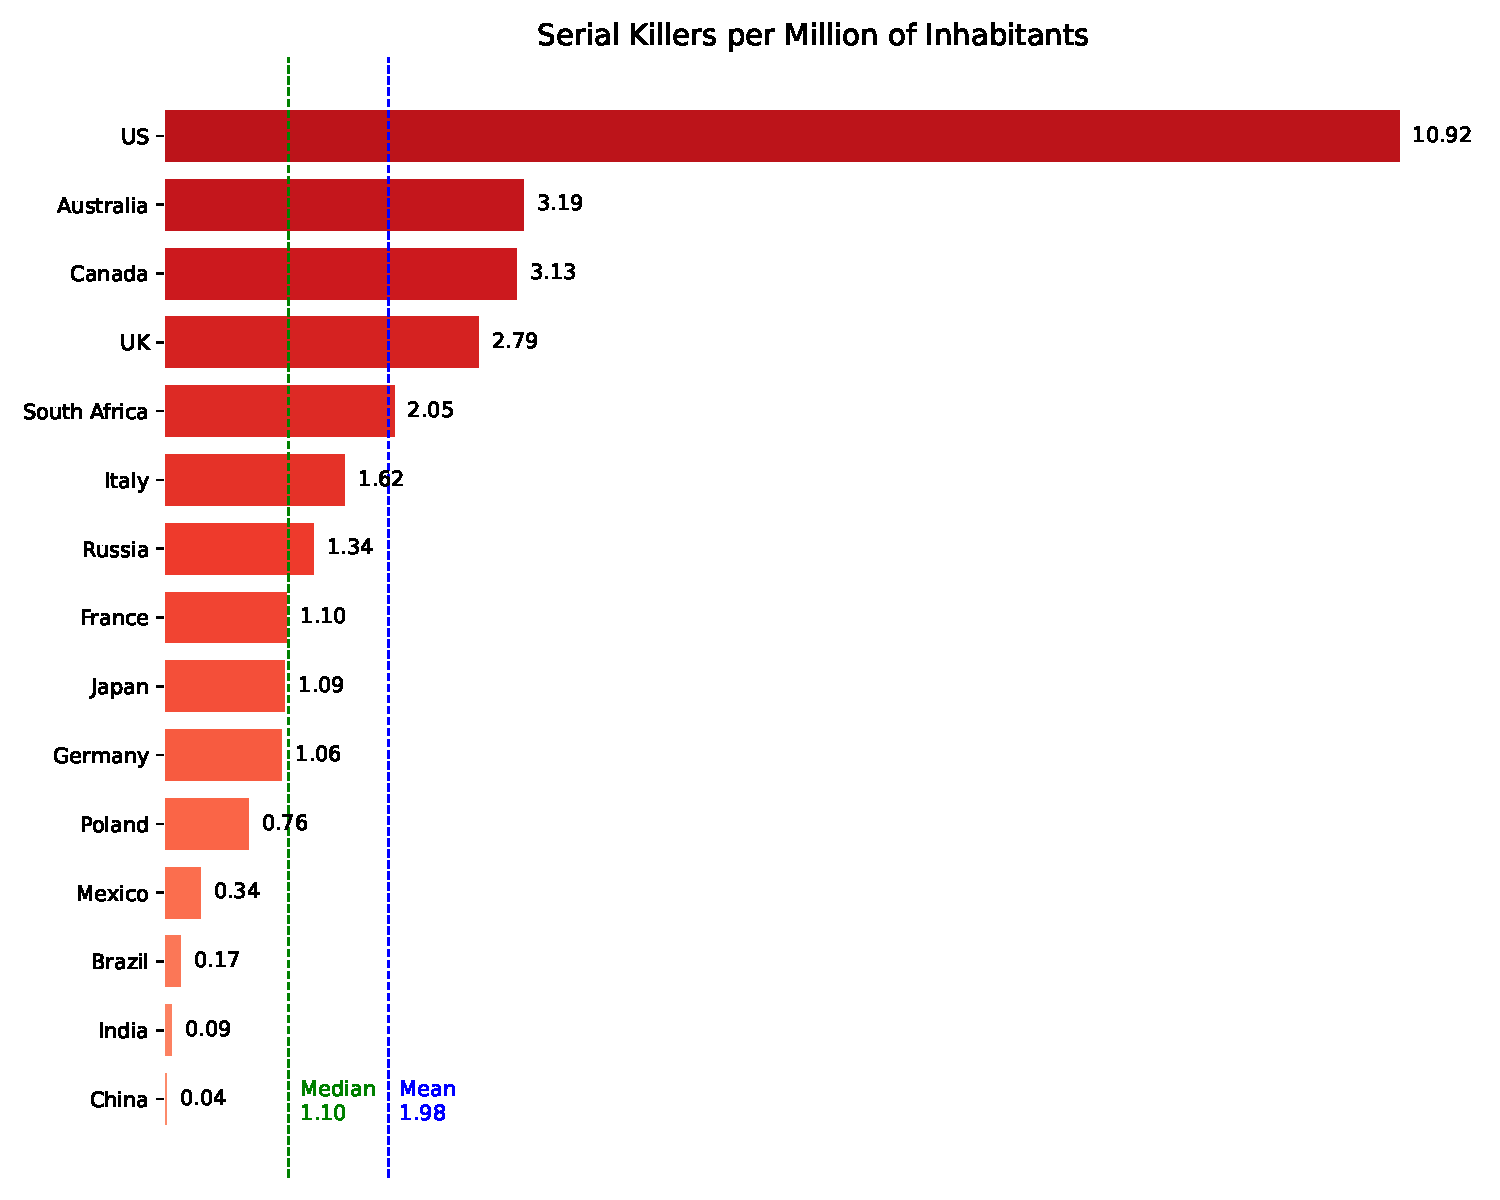
\includegraphics[width=0.7\textwidth]{Visualizations/serial_killers_per_million.pdf} % Replace with your file name
    \caption{Improved version of the bad visualization, Source\cite{worldatlas2025serialkillers}}
    \label{fig:improved}
\end{figure}

\subsection{Task 3: Good Visualization Critique}
\begin{figure}[H]
    \centering
    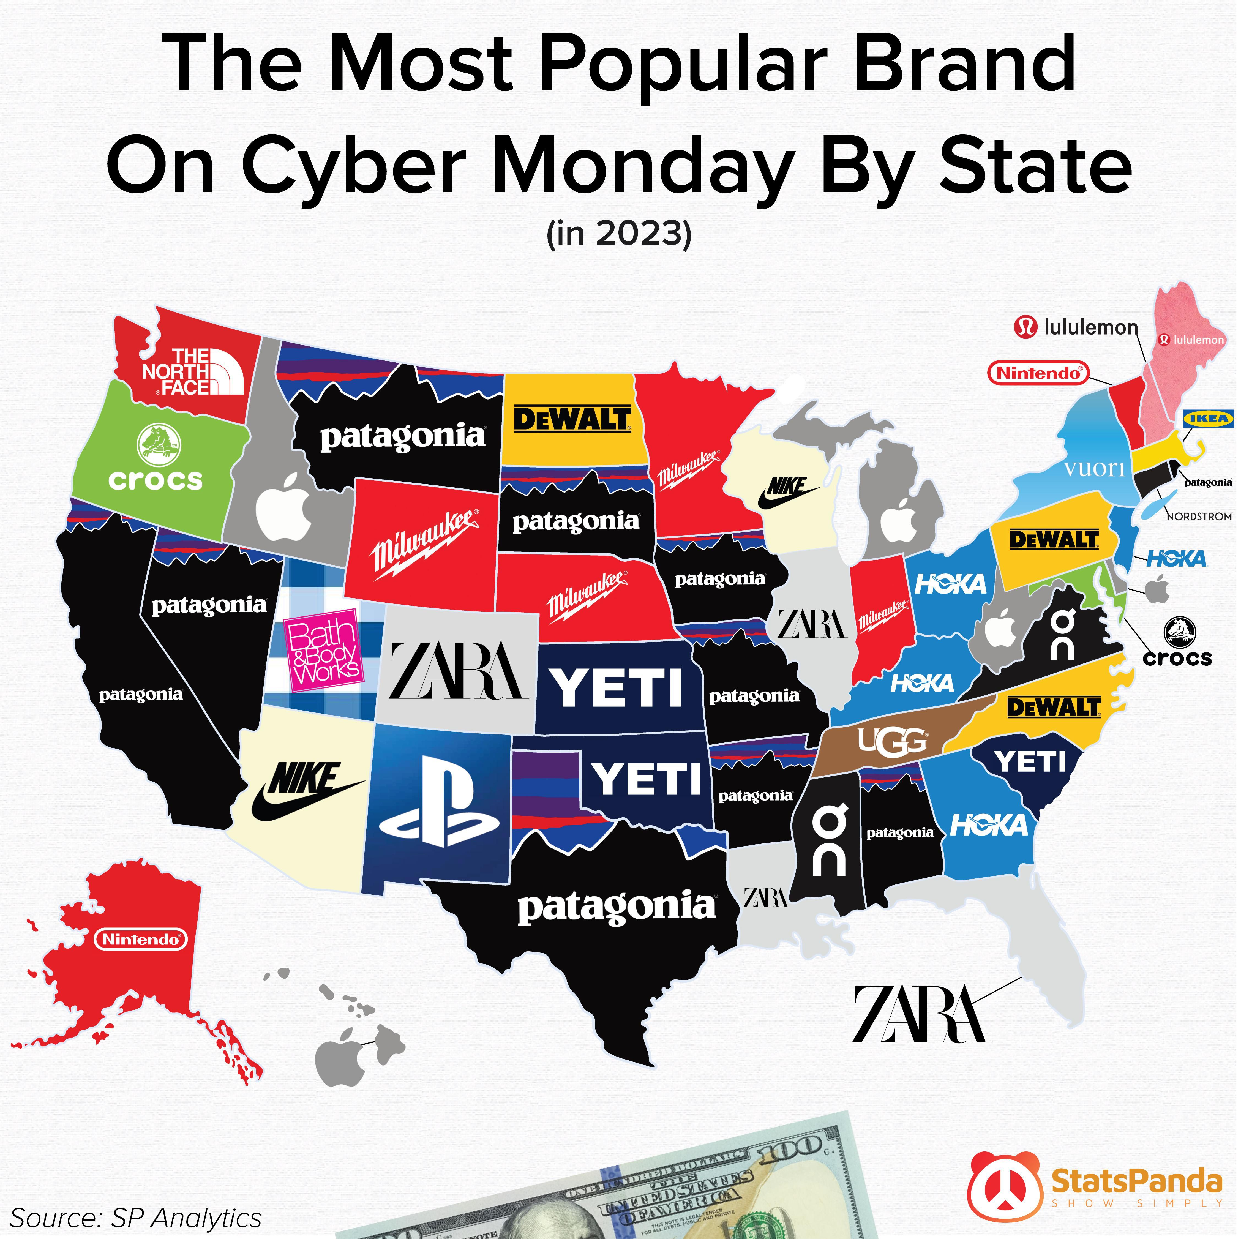
\includegraphics[width=0.5\textwidth]{Visualizations/good-data.pdf} % Replace with your file name
    \caption{Good Visualization, Source \cite{reddit2025cyberbrands}}
    \label{fig:good}
\end{figure}
\subsubsection{Critique}
The visualization is clear at first look. The observer does not need to carefully read any axis or legend. Thanks to the prominent title, the theme of the visualization is easily recognizable, and the recognizable logos make its interpretability straightforward. The colors utilized are associated with the brands and differ from one another, emphasizing the state shapes and enhancing engagement. This visualization is perfect for the general public, as it is simple and colorful. More importantly, it avoids complex data such as numbers or units of measurement, making the message elementary and direct. If it were accompanied by another visualization with more specific data or had an interactive element allowing users to overlay and access additional data, the visualization could be perfect.

\subsection{Task 4: Climate Change Visualization for Social Media}
\subsubsection{The Ozone Layer: Evidence of Global Environmental Action}

\begin{figure}[H]
    \centering
    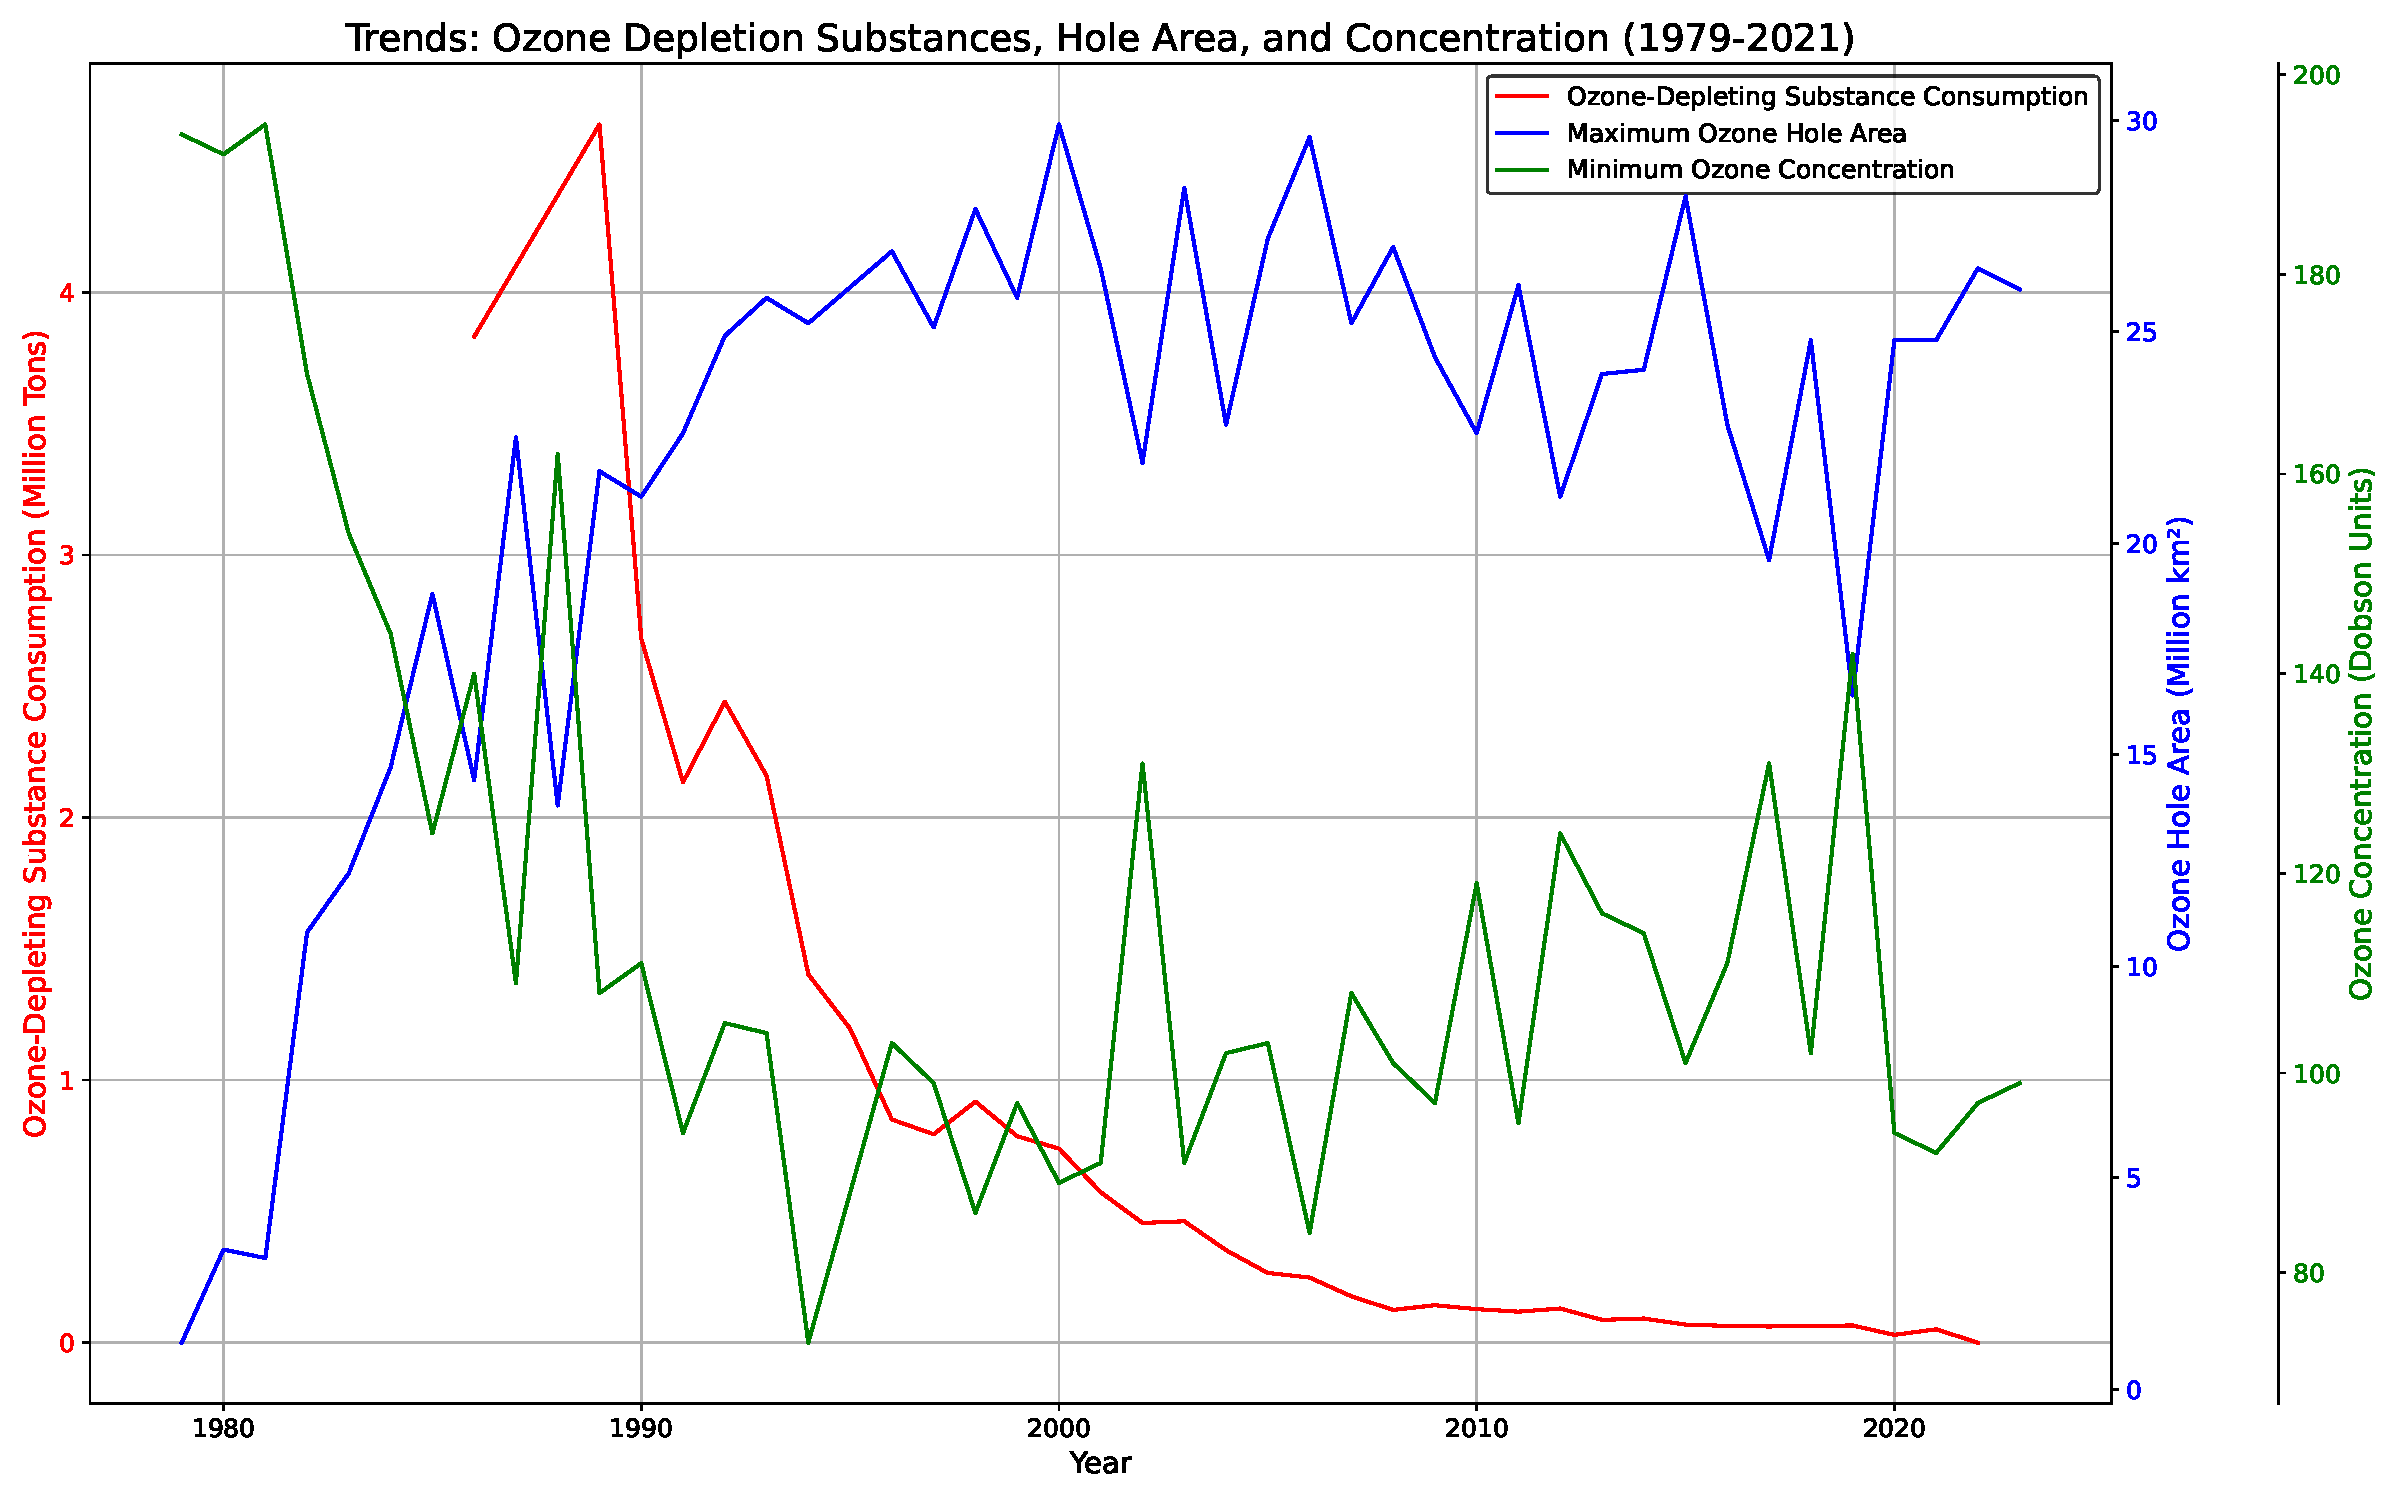
\includegraphics[width=0.8\textwidth]{Visualizations/ozone_data_visualization_t4.pdf} % Replace with your file name
    \caption{Climate change visualization for social media, Source \cite{nasa2024ozone}}
    \label{fig:climate}
\end{figure}

\subsubsection{LinkedIn Post: Healing the Ozone – A Lesson for Climate Change}

\textbf{What is the ozone layer, and why does it matter?}  \\
The ozone layer is the earths protective shield from the sun, specifically, the suns dangerous ultraviolet (UV) rays. Without it there would be serious consequences for life on Earth, for example a rise in skin cancer and ecological disruption!
 \\ \\ 
\textbf{A brief story of the ozone crisis:} \\
Very recently, in the 20th century, a massive hole in the ozone layer appeared primary over Antarctica. This was caused by a chemicals like chlorofluorocarbons (CFCs), more generally called ozone depleting substances. In 1987 the Montreal Protocol brought countries together to combat this dangerous phenomenon. 
As shown in the graph, after this protocol was introduced, the emissions of ozone harming substances finally declined and the ozone hole stabilized. 
The Montreal Protocol remained one of the greatest environmental successes, proving that global action can solve even the biggest challenges.
\\ \\
\textbf{Climate change lessons:} \\
The data in the visualization tells a crucial story! While the ozone layers destruction was rapid, its healing is significantly slower, and the ozone hole itself persists... This serves as a clear reminder for:
\begin{itemize}
    \item We alone as a species, we hold the power to both harm and heal environment
    \item Combating climate crisis like global warming requires unconditional global collaboration
    \item the healing process of nature is gradual and perhaps irreparable, which makes it even more important we do not make any more mistakes
\end{itemize}
 I call you to action: before the window of opportunity closes, let's take bold actions to address climate change, just as we did with the reduction of ozone depletion substances. We can guarantee a more sustainable and healthy Earth for us and coming generations, if we work together!


\subsection{Task 5: Black-and-White Visualization}
\subsubsection{Correlation between GDP of Nigeria and U.S. Crude Oil Price Over Time}

\begin{figure}[H]
    \centering
    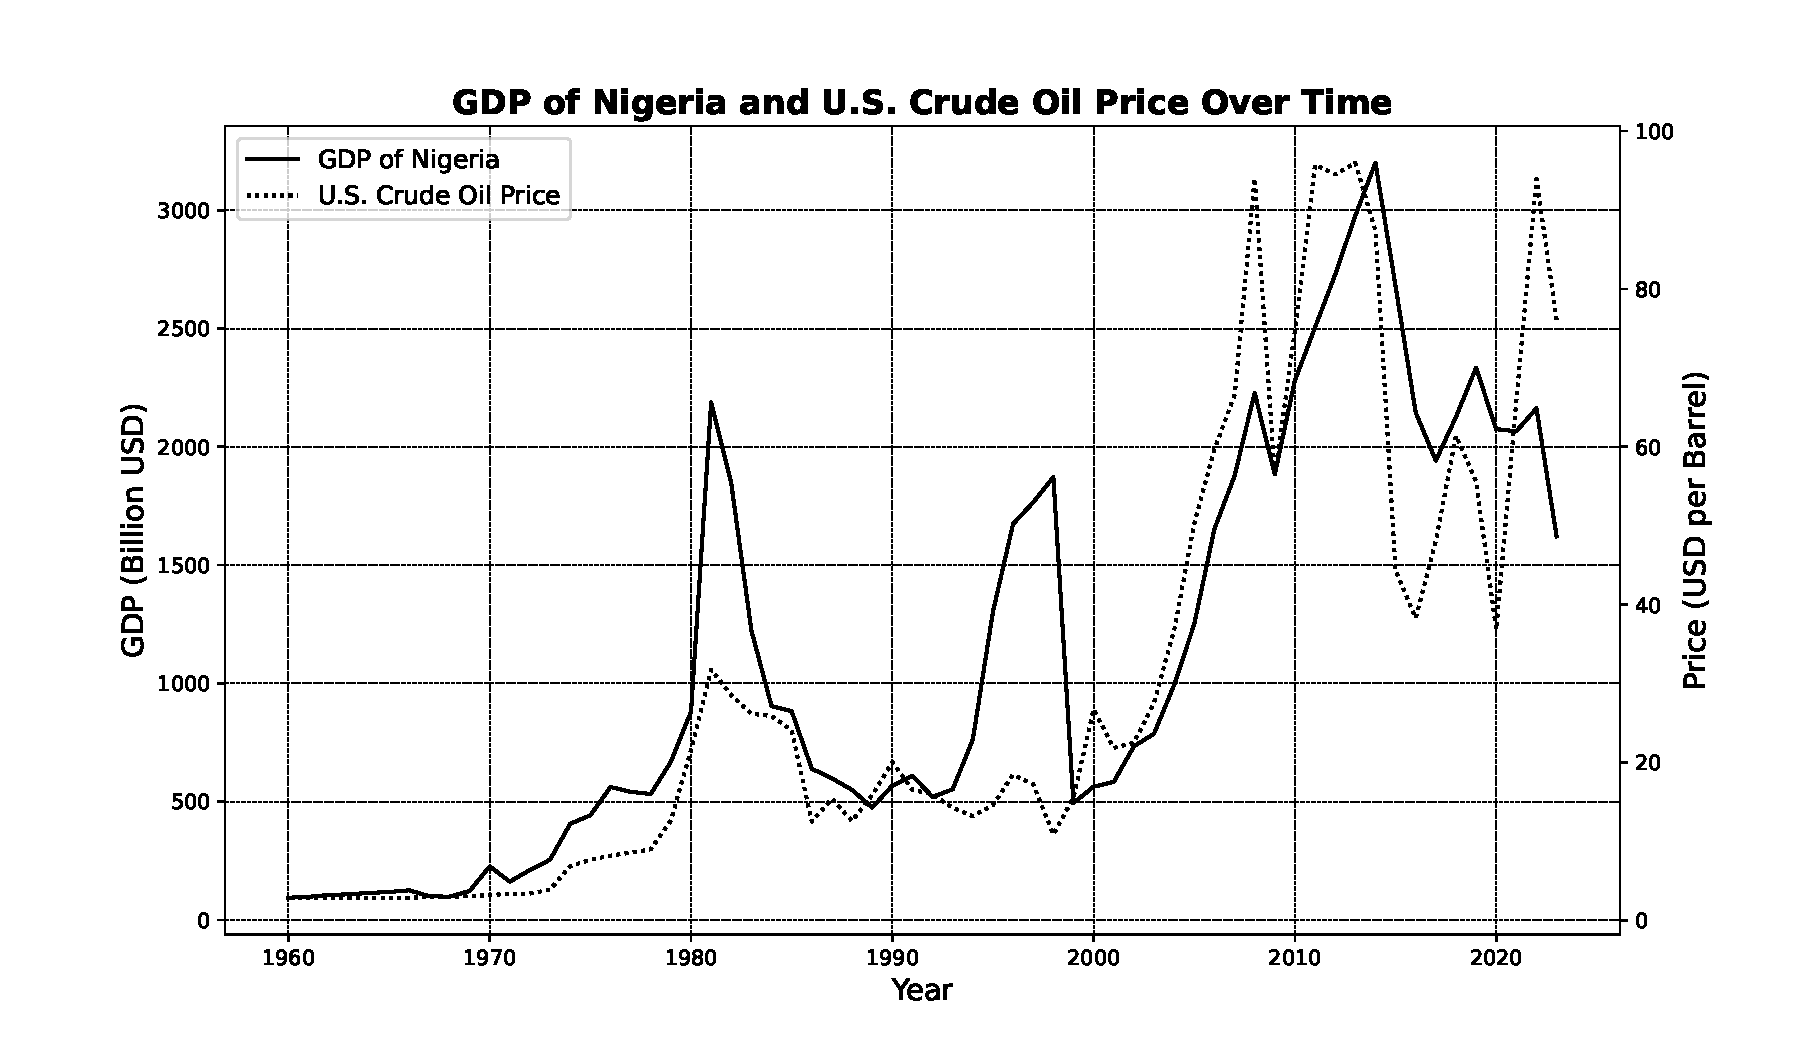
\includegraphics[width=0.9\textwidth]{Visualizations/GDP_Oil_Price.pdf} % Replace with your file name
    \caption{Black-and-white visualization, Sources \cite{eia2025petroleum} \cite{nigeriaGDP}}
    \label{fig:bw}
\end{figure}

\subsection{Task 6: Visualization with Color as a Key Aesthetic}
\subsubsection{Global Energy Consumption in 2023}

\begin{figure}[H]
    \centering
    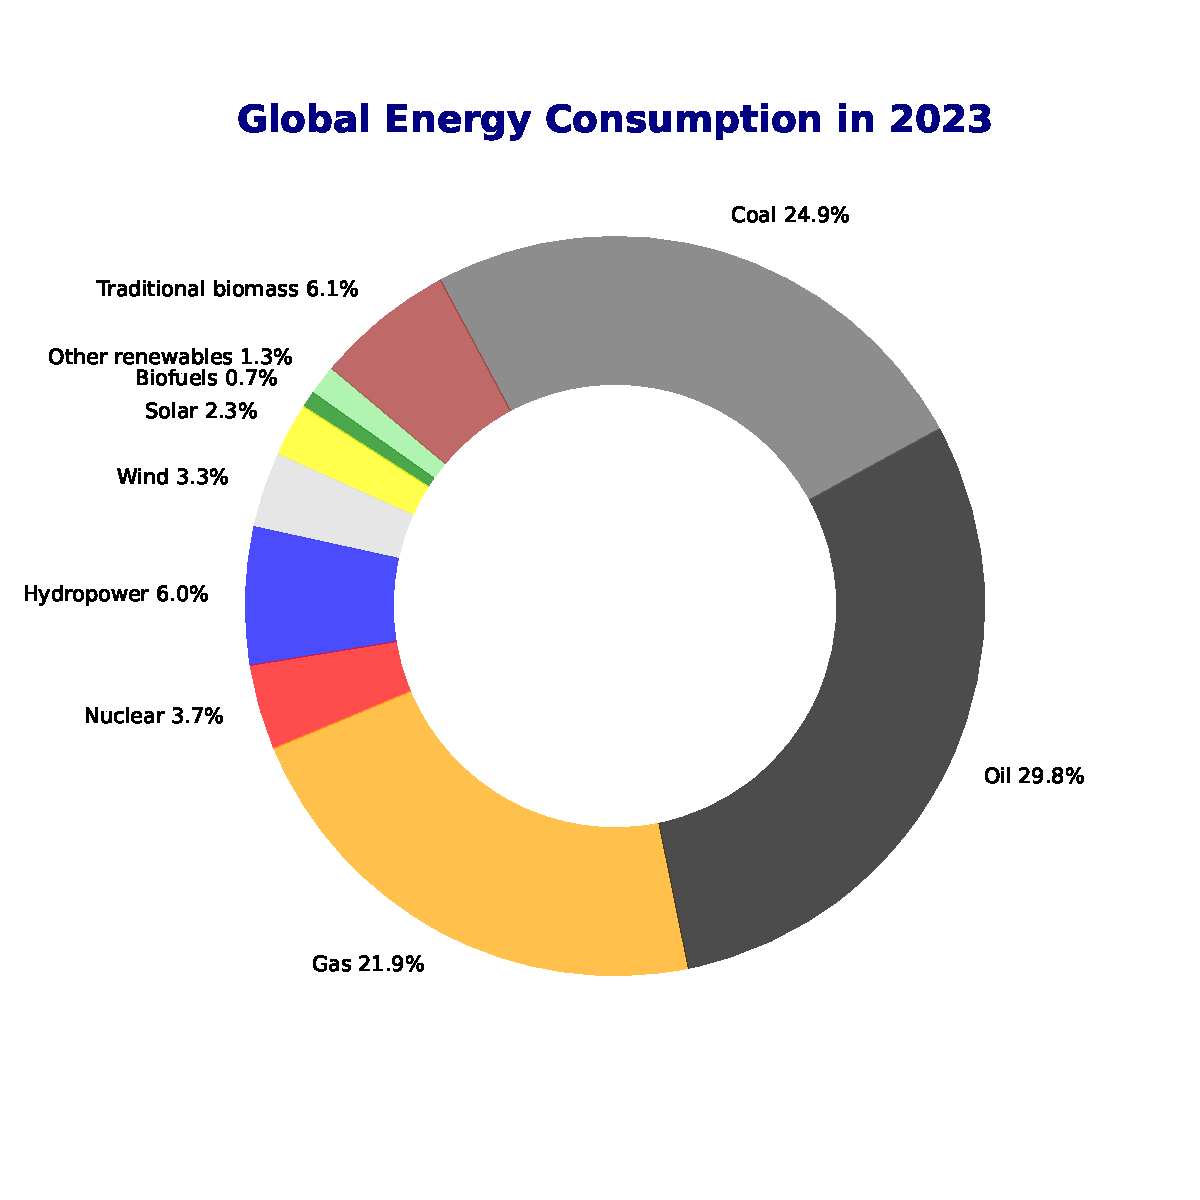
\includegraphics[width=0.5\textwidth]{Visualizations/energy_substitution_2023.pdf}% Replace with your file name
    \caption{Visualization utilizing color as a key aesthetic, Source \cite{ourworld2025energy}}
    \label{fig:color}
\end{figure}

\subsection{Task 7: Data-Ink Optimization Showcase}
\subsubsection{Energy Balance by Carrier in Switzerland in 2023}
\begin{figure}[H]
    \centering
    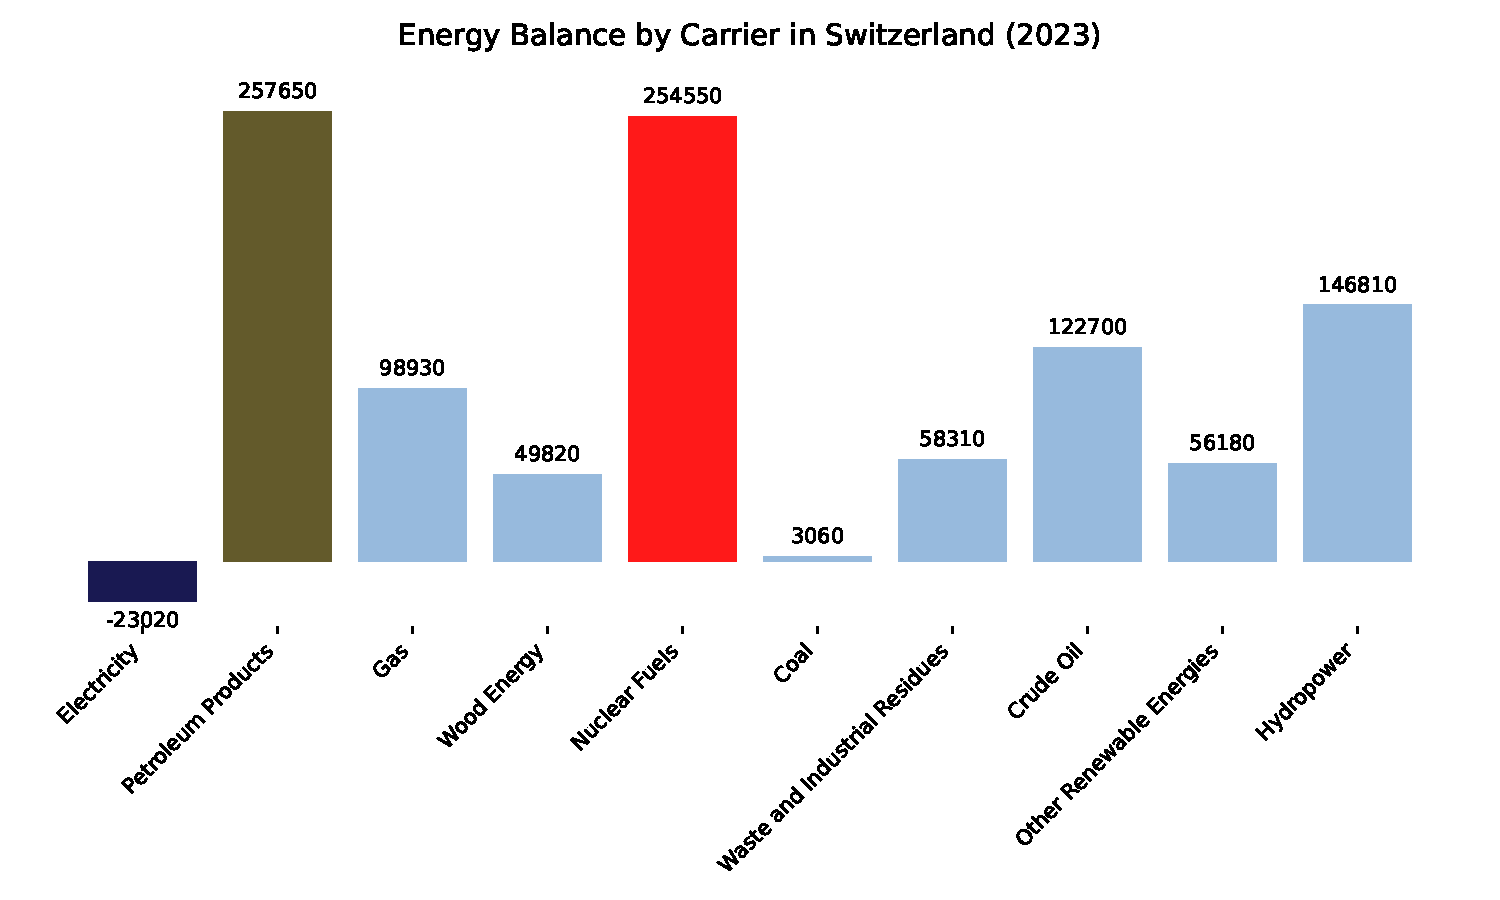
\includegraphics[width=0.7\textwidth]{Visualizations/energy_balance.pdf} % Replace with your file name
    \caption{Data-Ink optimization visualization, Source \cite{swiss2025energybalance}}
    \label{fig:swissbalanceenergy}
\end{figure}

\subsection{Task 8: Uncommon Visualization}
\subsubsection{Average American Expenditure in 2023}
\begin{figure}[H]
    \centering
    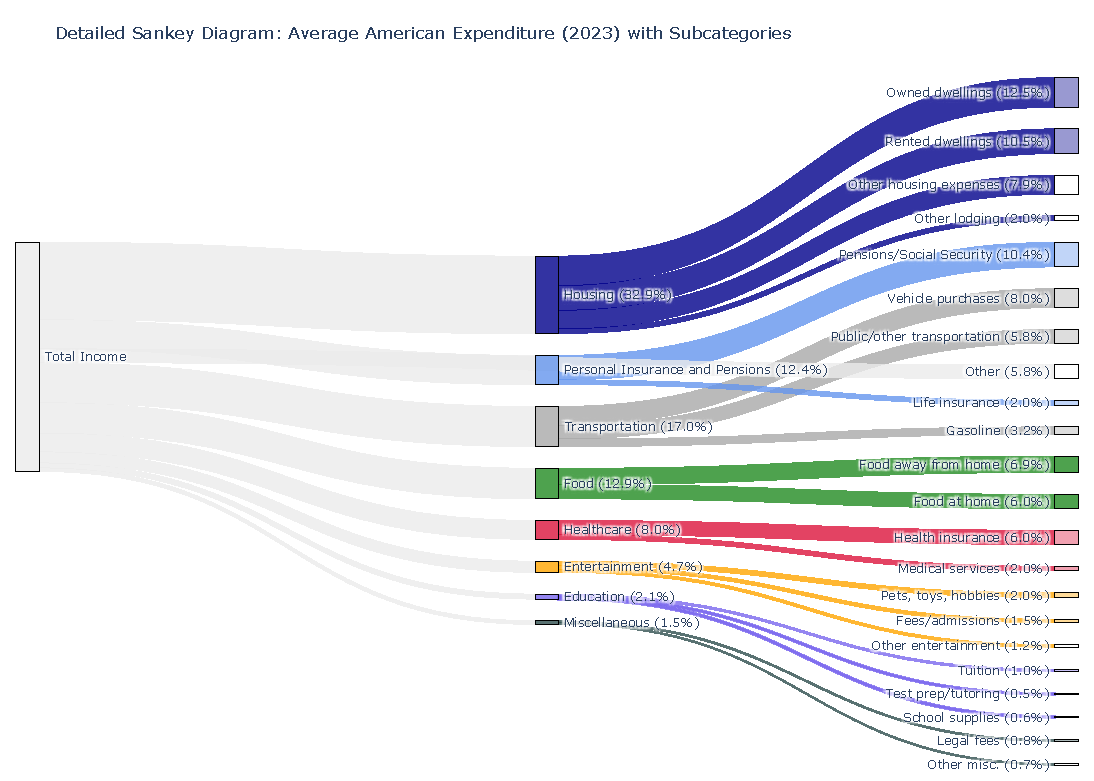
\includegraphics[width=0.7\textwidth]{Visualizations/sankey_diagram.pdf} % Replace with your file name
    \caption{Uncommon visualization, Source \cite{bls2025expenditure}}
    \label{fig:americanExp}
\end{figure}

\subsection{Task 9: Visualization by hand}
\subsection{Ionization Energy}
\begin{figure}[H]
    \centering
    \includegraphics[width=0.7\textwidth]{Visualizations/ionization.pdf} % Replace with your file name
    \caption{Visualization by hand, Source \cite{chemistrytalk2025ionization}}
    \label{fig:ionization}
\end{figure}


\subsection{Task 10: Visualization with ChatGPT Pro}
\subsection{Number of Free-to-use vs Pay-to-Use ATMs Over Time}
\begin{figure}[H]
    \centering
    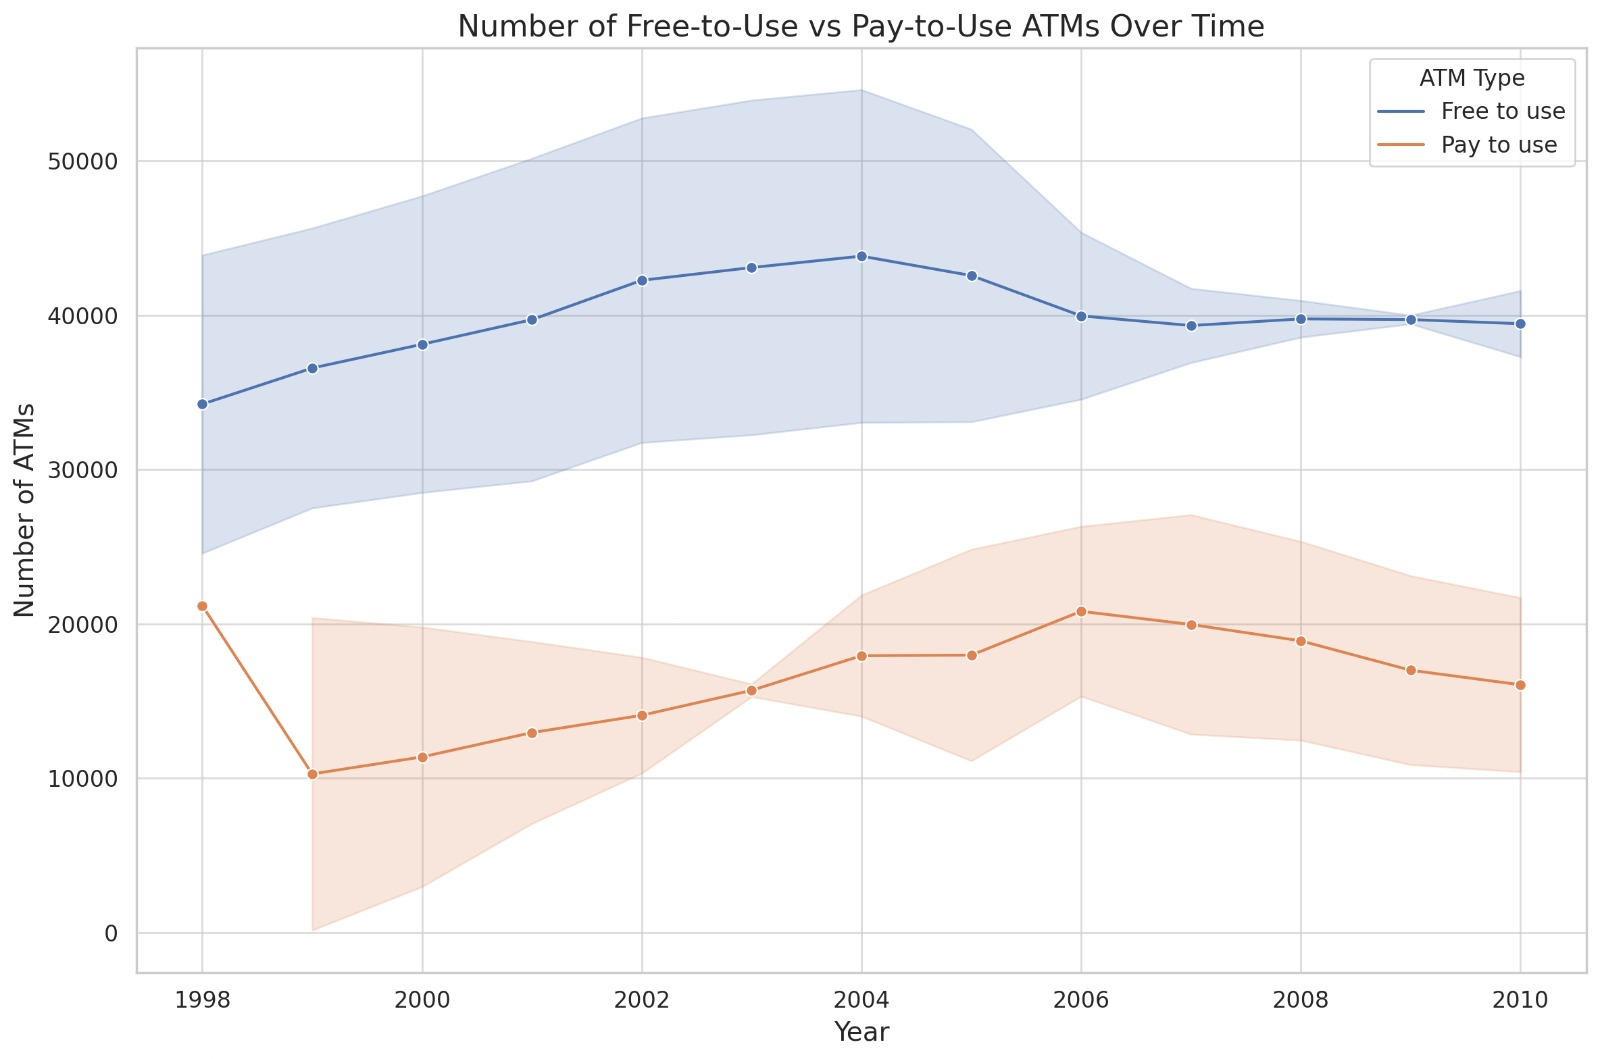
\includegraphics[width=0.8\textwidth]{plot.jpeg} % Replace with your file name
    \caption{Number of Free-to-use vs Pay-to-Use ATMs Over Time, Source \cite{gptplotATM}}
    \label{fig:GPT}
\end{figure}


\subsection{Task 11: Data Map}
\subsubsection{Inflation Rate in Europe in 2023}

\begin{figure}[H]
    \centering
    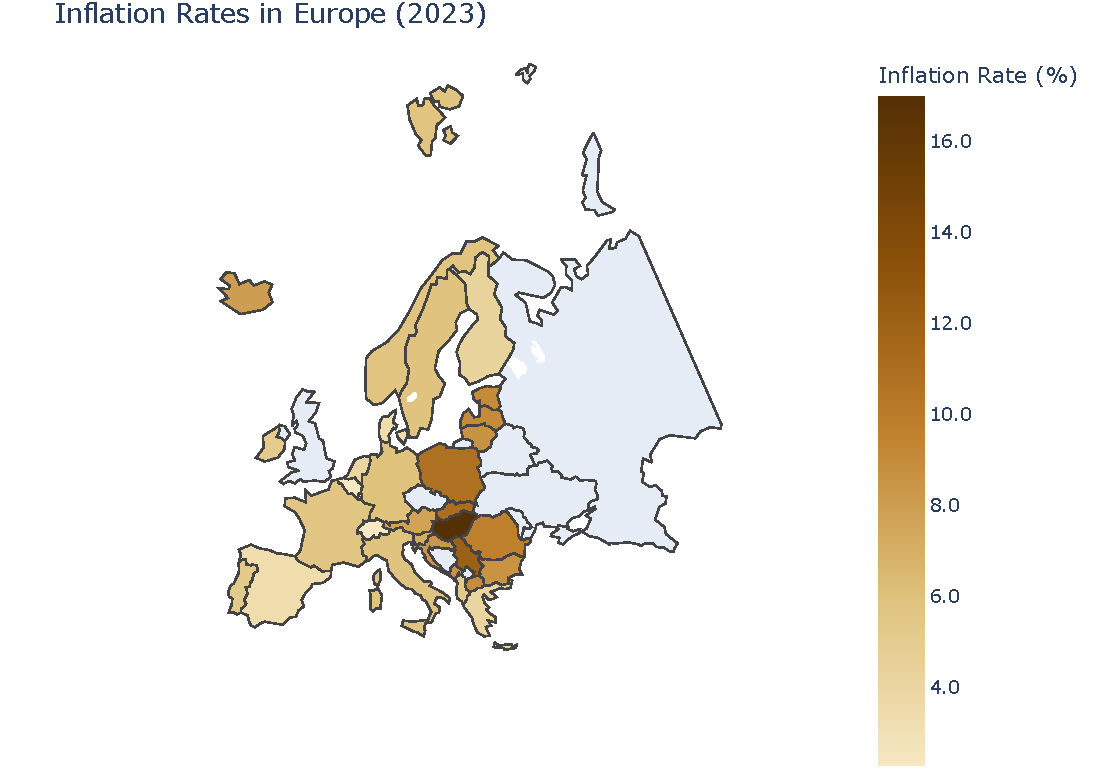
\includegraphics[width=0.7\textwidth]{Visualizations/europe_inflation_rates_2023.pdf} % Replace with your file name
    \caption{Inflation rate in Europe in 2023, Source \cite{eurostat2025inflation}}
    \label{fig:inflation}
\end{figure}

\subsection{Task 12: Interactive Visualization}
\subsection{Internet Fixed Broadband Subscriptions Over Time (1998-2022)}
\href{https://interactive-visualization.vercel.app/}{Visit URL to interact!}

\begin{figure}[H]
    \centering
    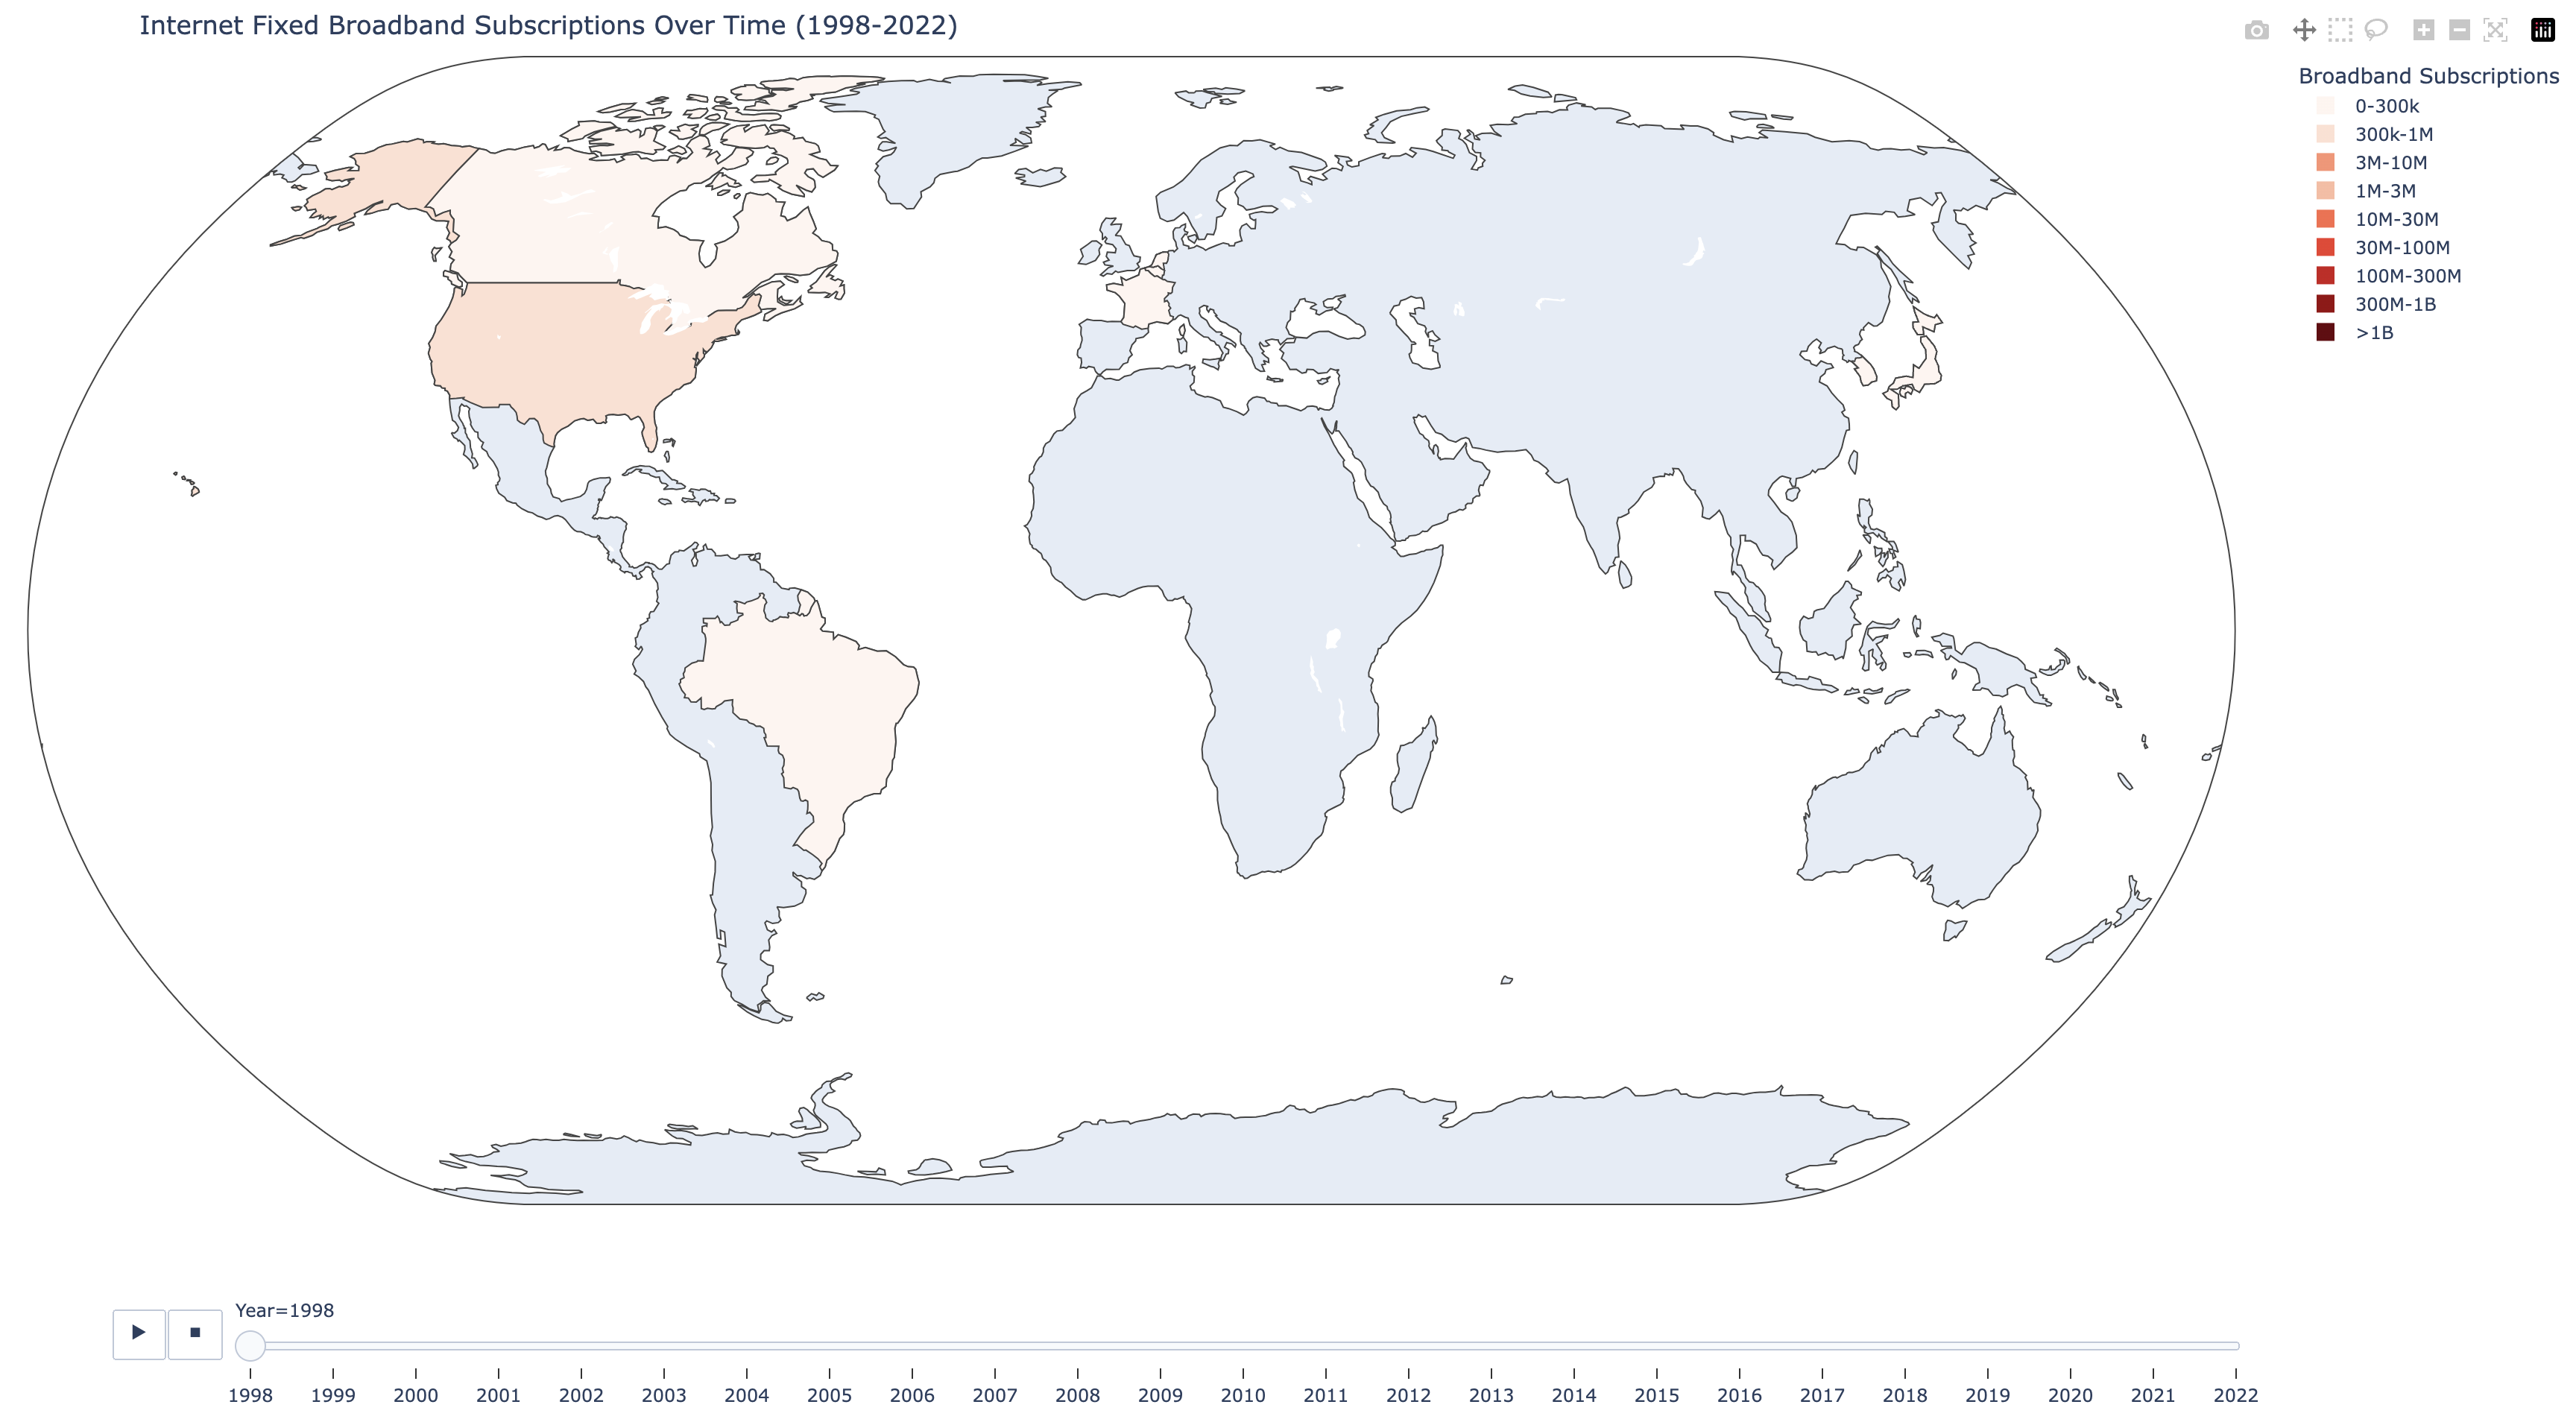
\includegraphics[width=0.9\textwidth]{Visualizations/Screenshot 2025-01-17 at 21.48.35.png} % Replace with your file name
    \caption{Source \cite{ourworldinternet2025}}
    \label{fig:interactive1}
\end{figure}
\begin{figure}[H]
    \centering
    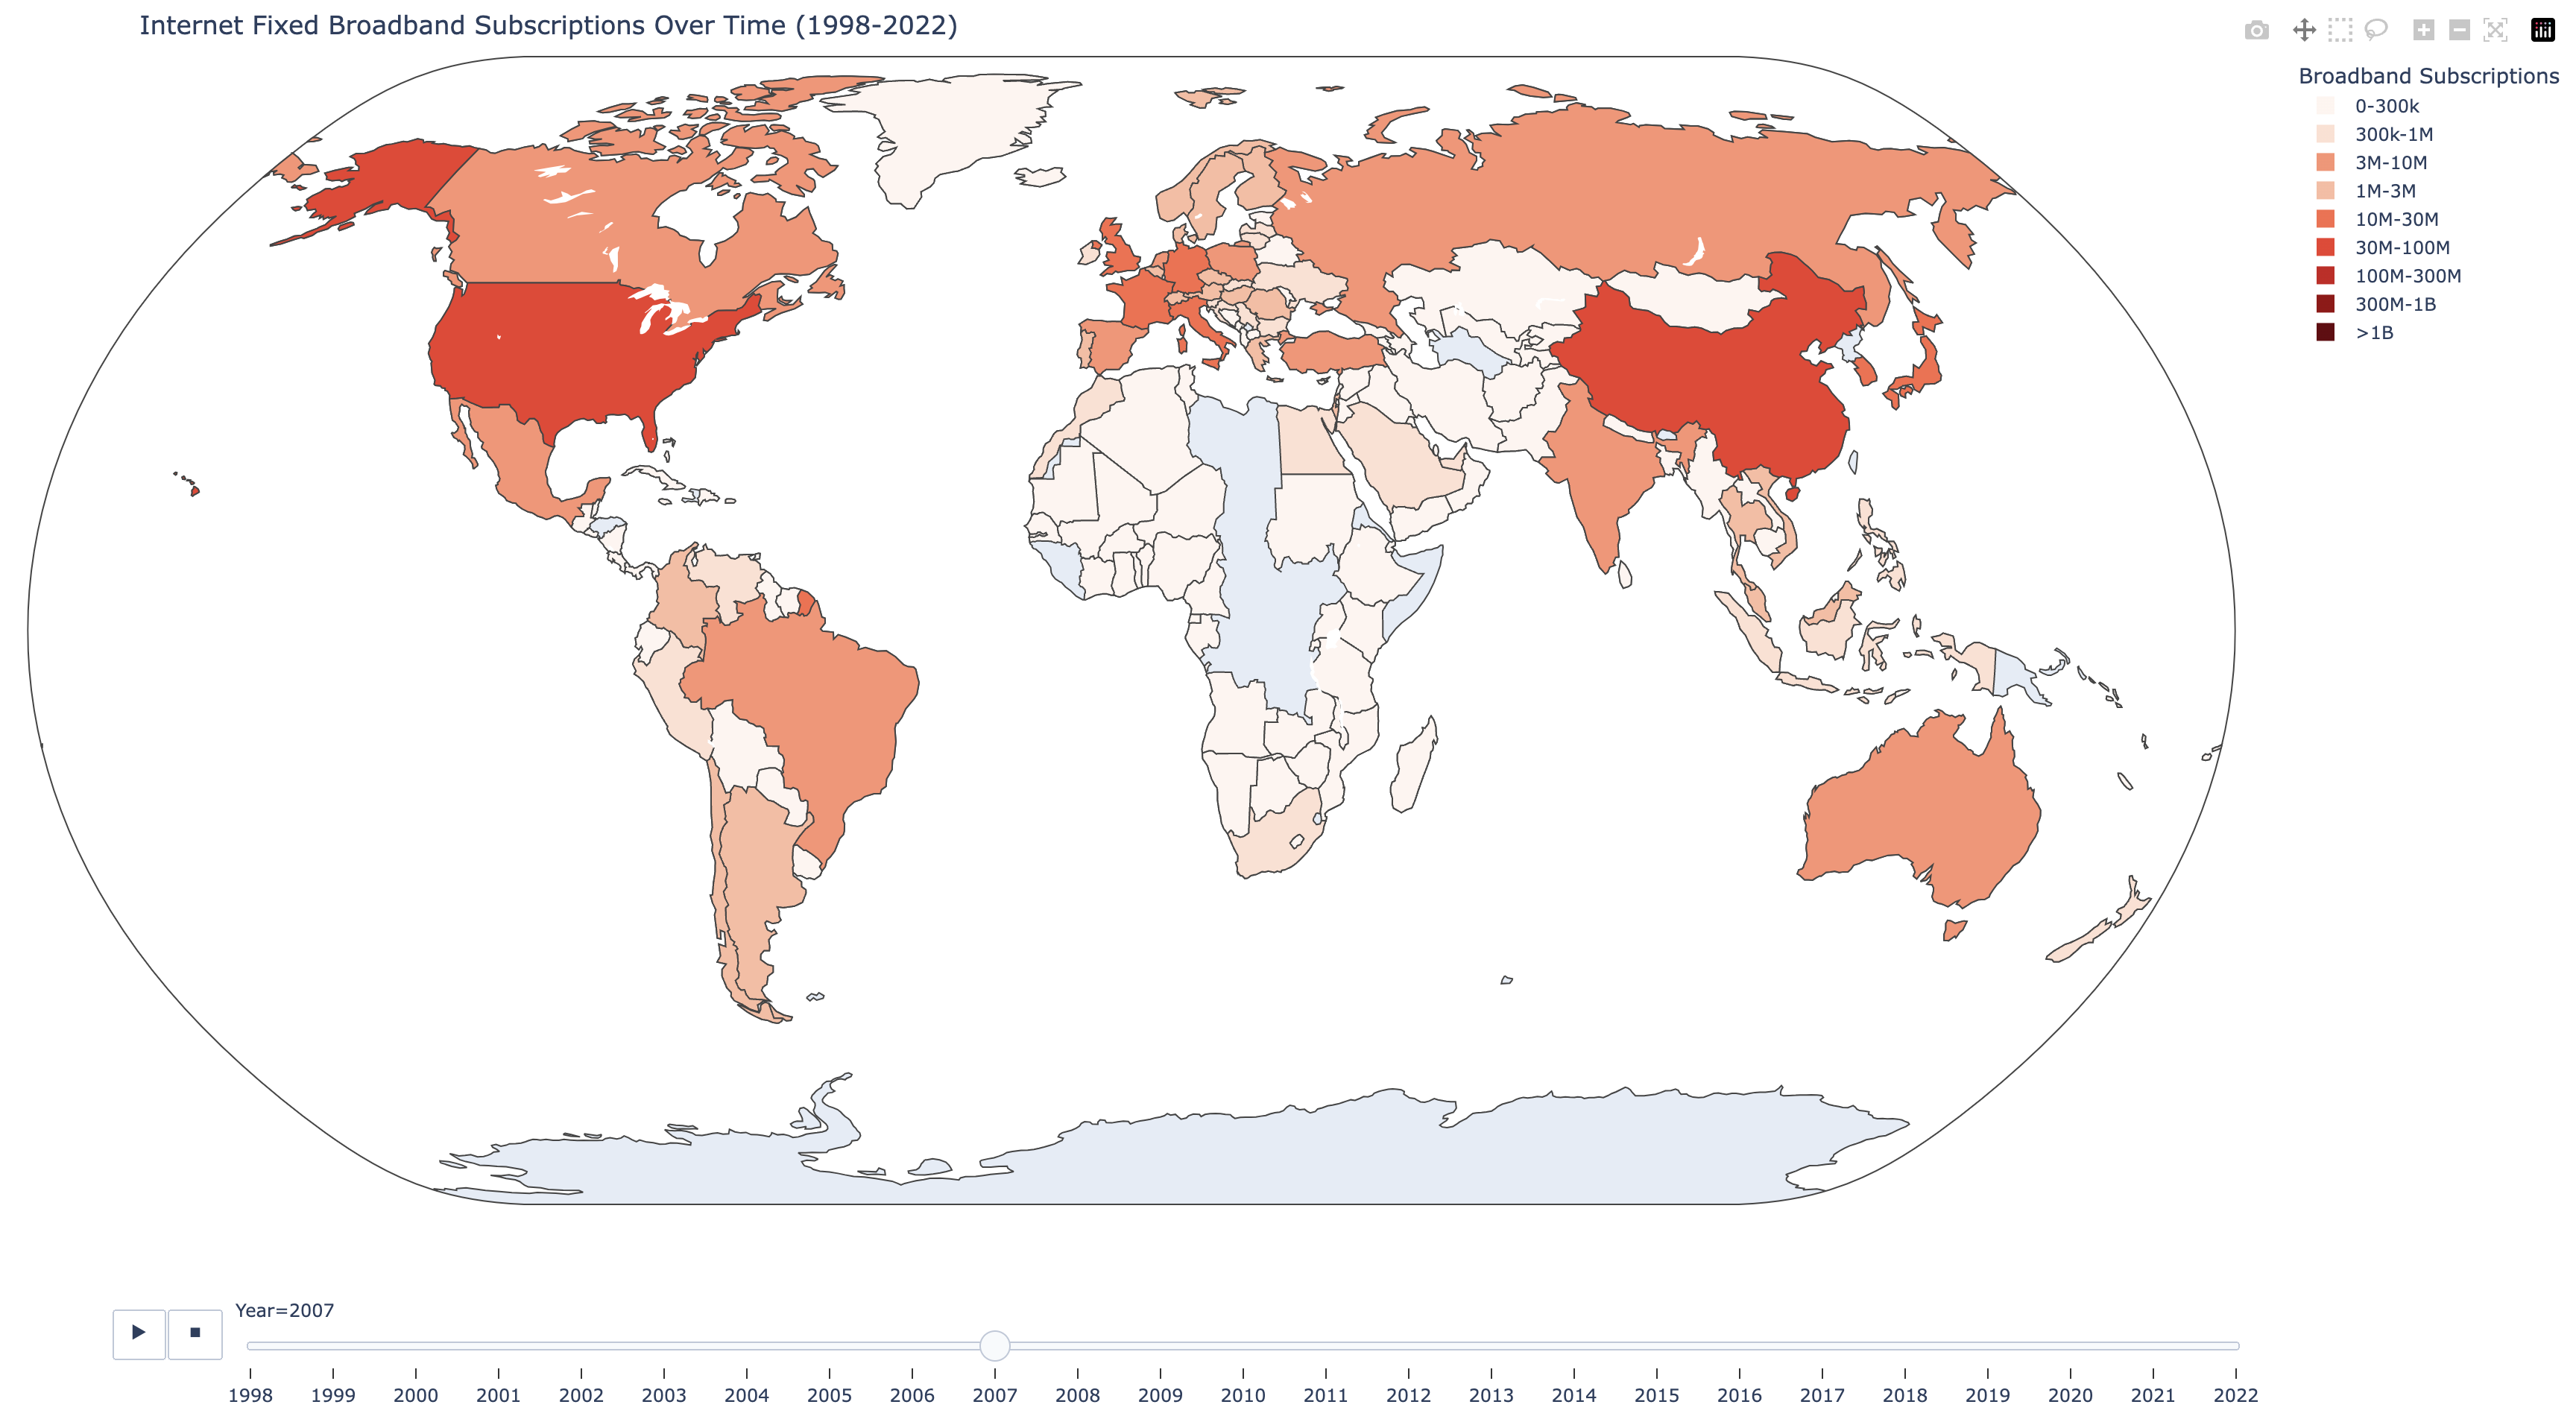
\includegraphics[width=0.9\textwidth]{Visualizations/Screenshot 2025-01-17 at 21.49.00.png} % Replace with your file name
    \caption{Source \cite{ourworldinternet2025}}
    \label{fig:interactive2}
\end{figure}
\begin{figure}[H]
    \centering
    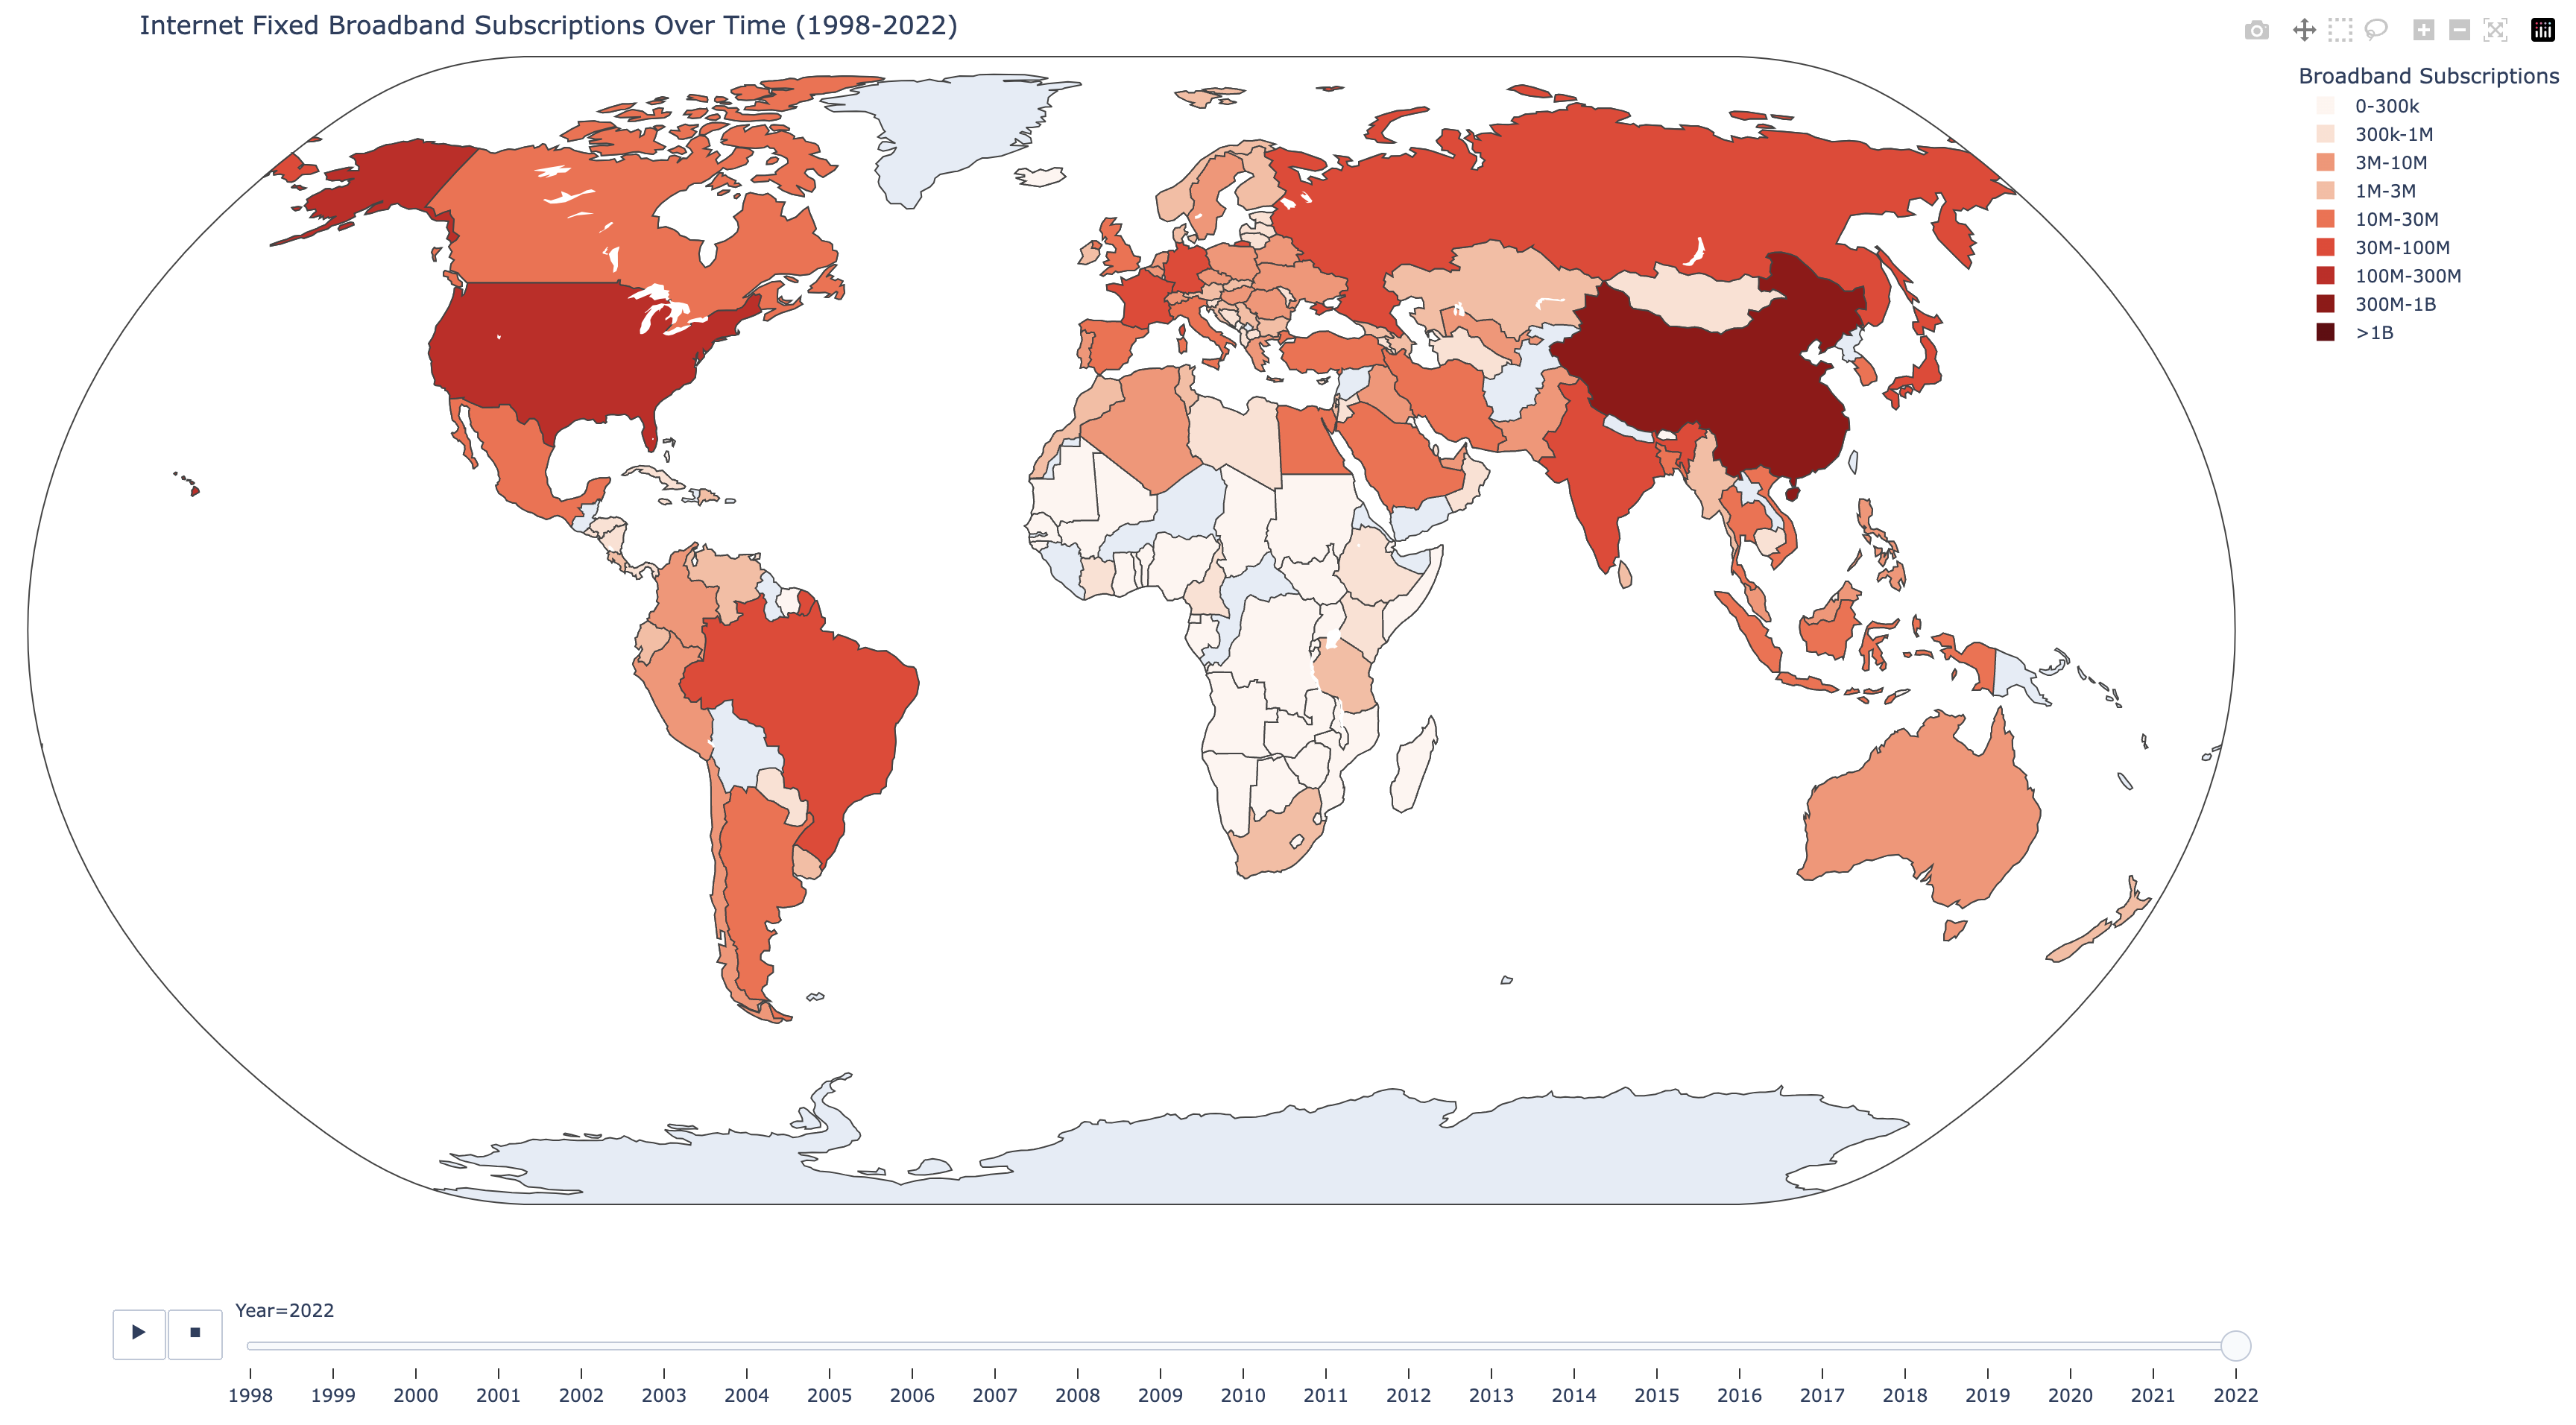
\includegraphics[width=0.9\textwidth]{Visualizations/Screenshot 2025-01-17 at 21.49.12.png} % Replace with your file name
    \caption{Source \cite{ourworldinternet2025}}
    \label{fig:interactive3}
\end{figure}

\subsection{Task 13: Creation Process of "GDP of Nigeria and U.S. Crude Oil Price Over Time"}
\subsubsection{Sketch}
\begin{figure}[H]
    \centering
    \includegraphics[width=0.6\textwidth]{Visualizations/NIGERIA GDP VS US CRUDE OIL PRICE.pdf} % Replace with your file name
    \caption{Sketch}
    \label{fig:sketch}
\end{figure}
My idea was to show the dependency of the Nigerian GDP on the price of the crude oil. The inspiration came from a \href{https://www.youtube.com/watch?v=SnqLPSCWads}{YouTube video} I watched one years ago and I wanted to present the concept in this visualization.

\newpage

\subsubsection{Version 1}
I started by searching on the web for the GPD of Nigeria. With assistance of ChatGPT I cleaned the dataset from missing values and typos and plotted it.
\begin{figure}[H]
    \centering
    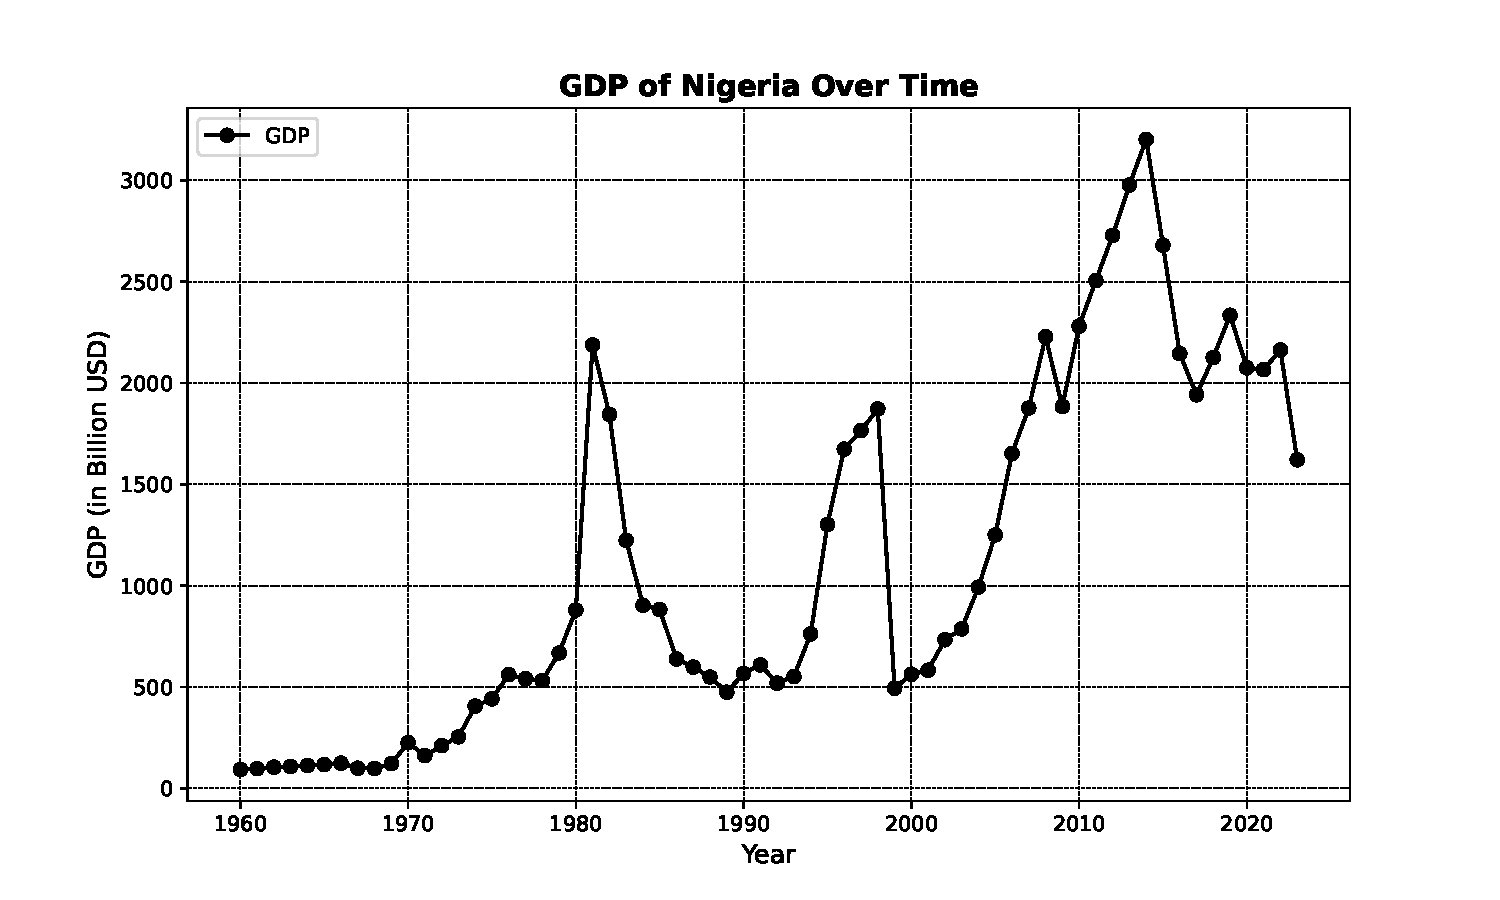
\includegraphics[width=0.8\textwidth]{Visualizations/1.pdf} % Replace with your file name
    \caption{Version 1}
    \label{fig:1}
\end{figure}

\newpage
\subsubsection{Version 2}

Then I added the crude oil prices after having a little trouble finding a reliable dataset with enough years of data. The result is better than expected, now I have data from the 19th century.
\begin{figure}[H]
    \centering
    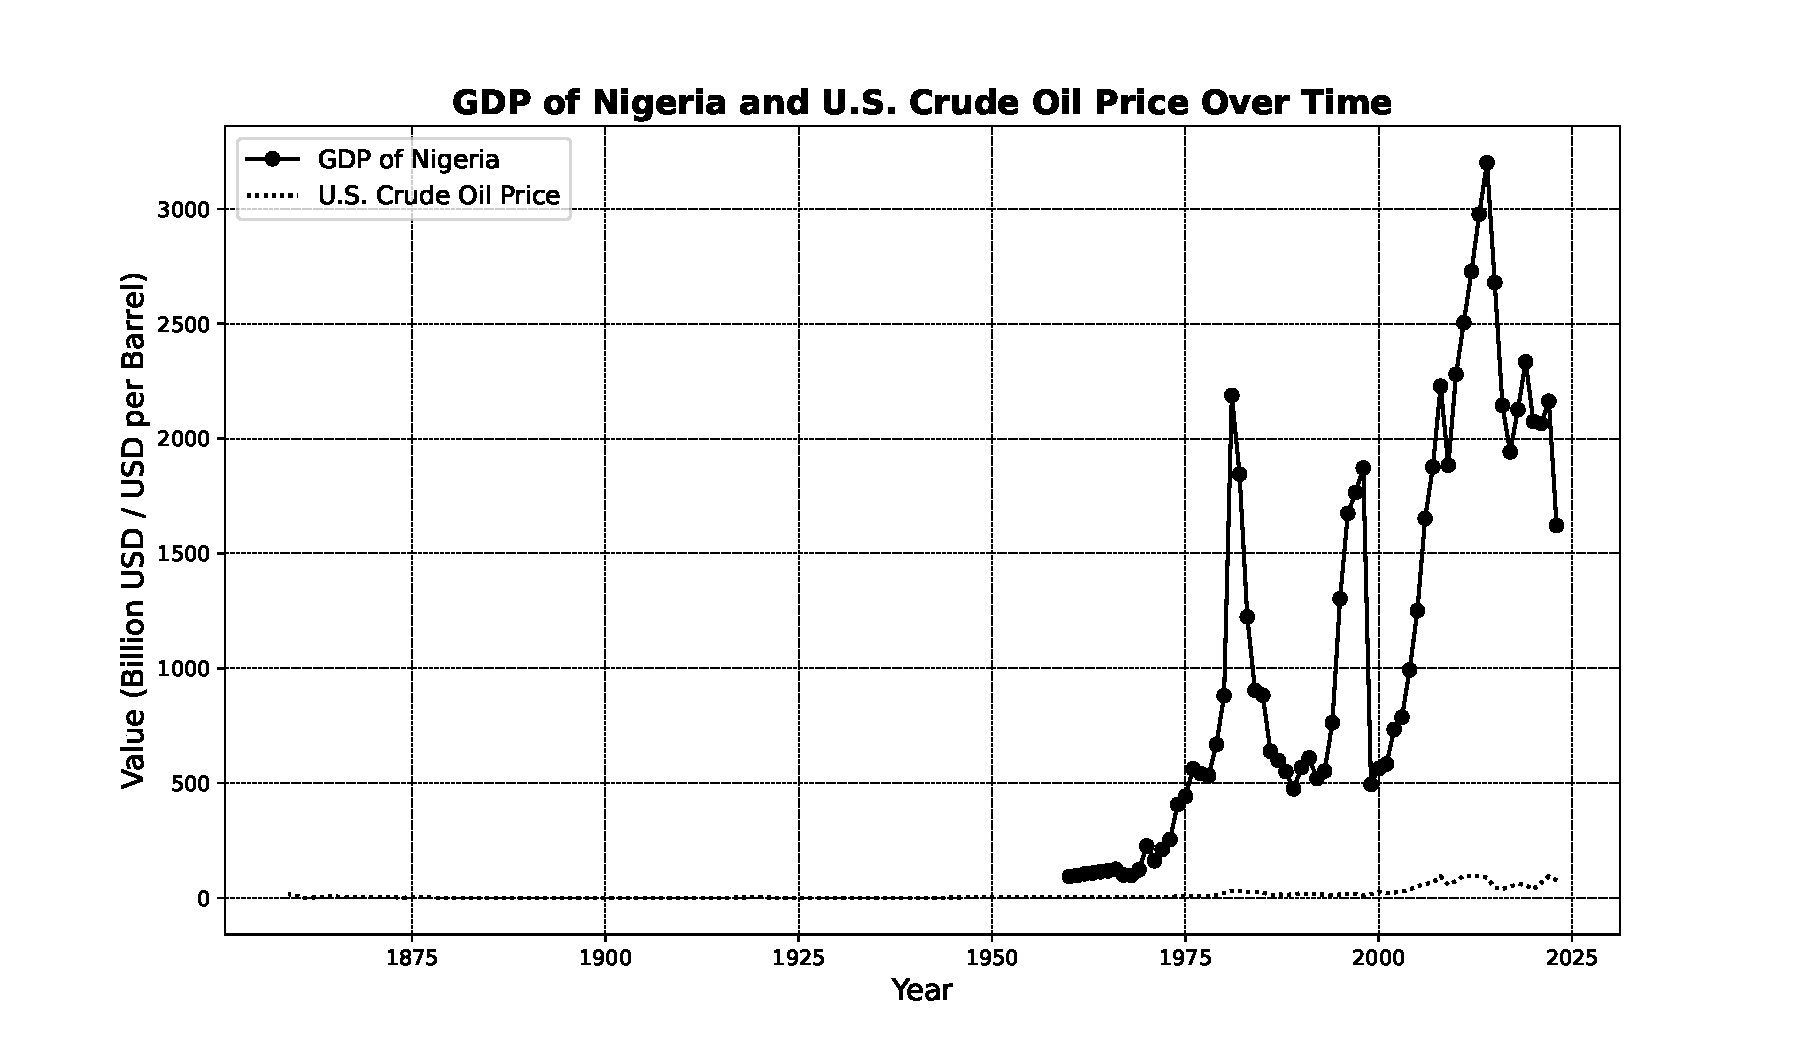
\includegraphics[width=0.8\textwidth]{Visualizations/3.pdf} % Replace with your file name
    \caption{Version 2}
    \label{fig:2}
\end{figure}

\subsubsection{Version 3}
 I limited the time frame to the years where I have data for both lines. I wanted to keep only one scale for axis, thus I played around to fix the scaling of the y-axis, with poor results. I started to realize that I would have been better to sacrifice simplicity to have a better data visualization like figure \ref{fig:climate}.
\begin{figure}[H]
    \centering
    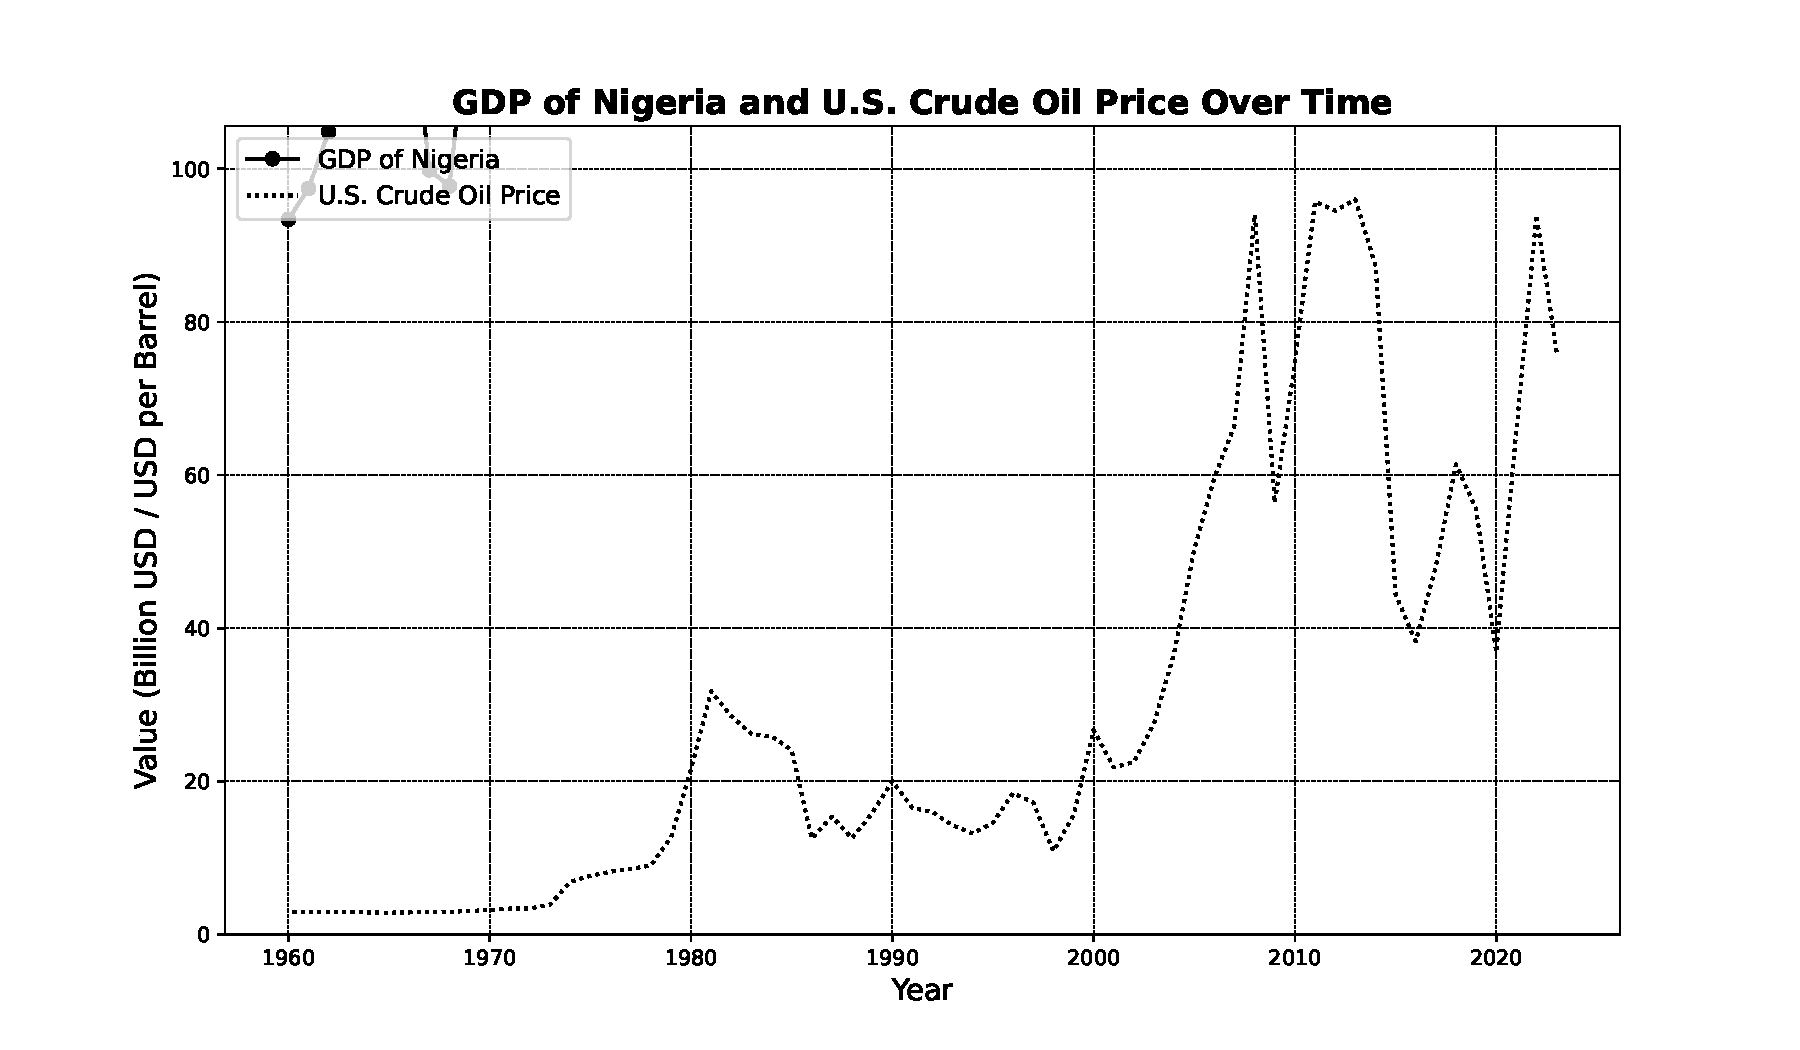
\includegraphics[width=0.7\textwidth]{Visualizations/2linesfar.pdf} % Replace with your file name
    \caption{}
    \label{fig:3}
\end{figure}

\subsubsection{Final Version}
For the final version of the visualization I removed the data points to have only lines, added an additional scale on the y-axis on the right of the plot and most importantly fixed the latter in order to have the two lines moving together and not one flat line and another showing the trend. See result at figure \ref{fig:bw}.

\newpage

\subsection{Task 14: More Visualizations}
\subsubsection{Measures history of Gravitational Constant G}

\begin{figure}[H]
    \centering
    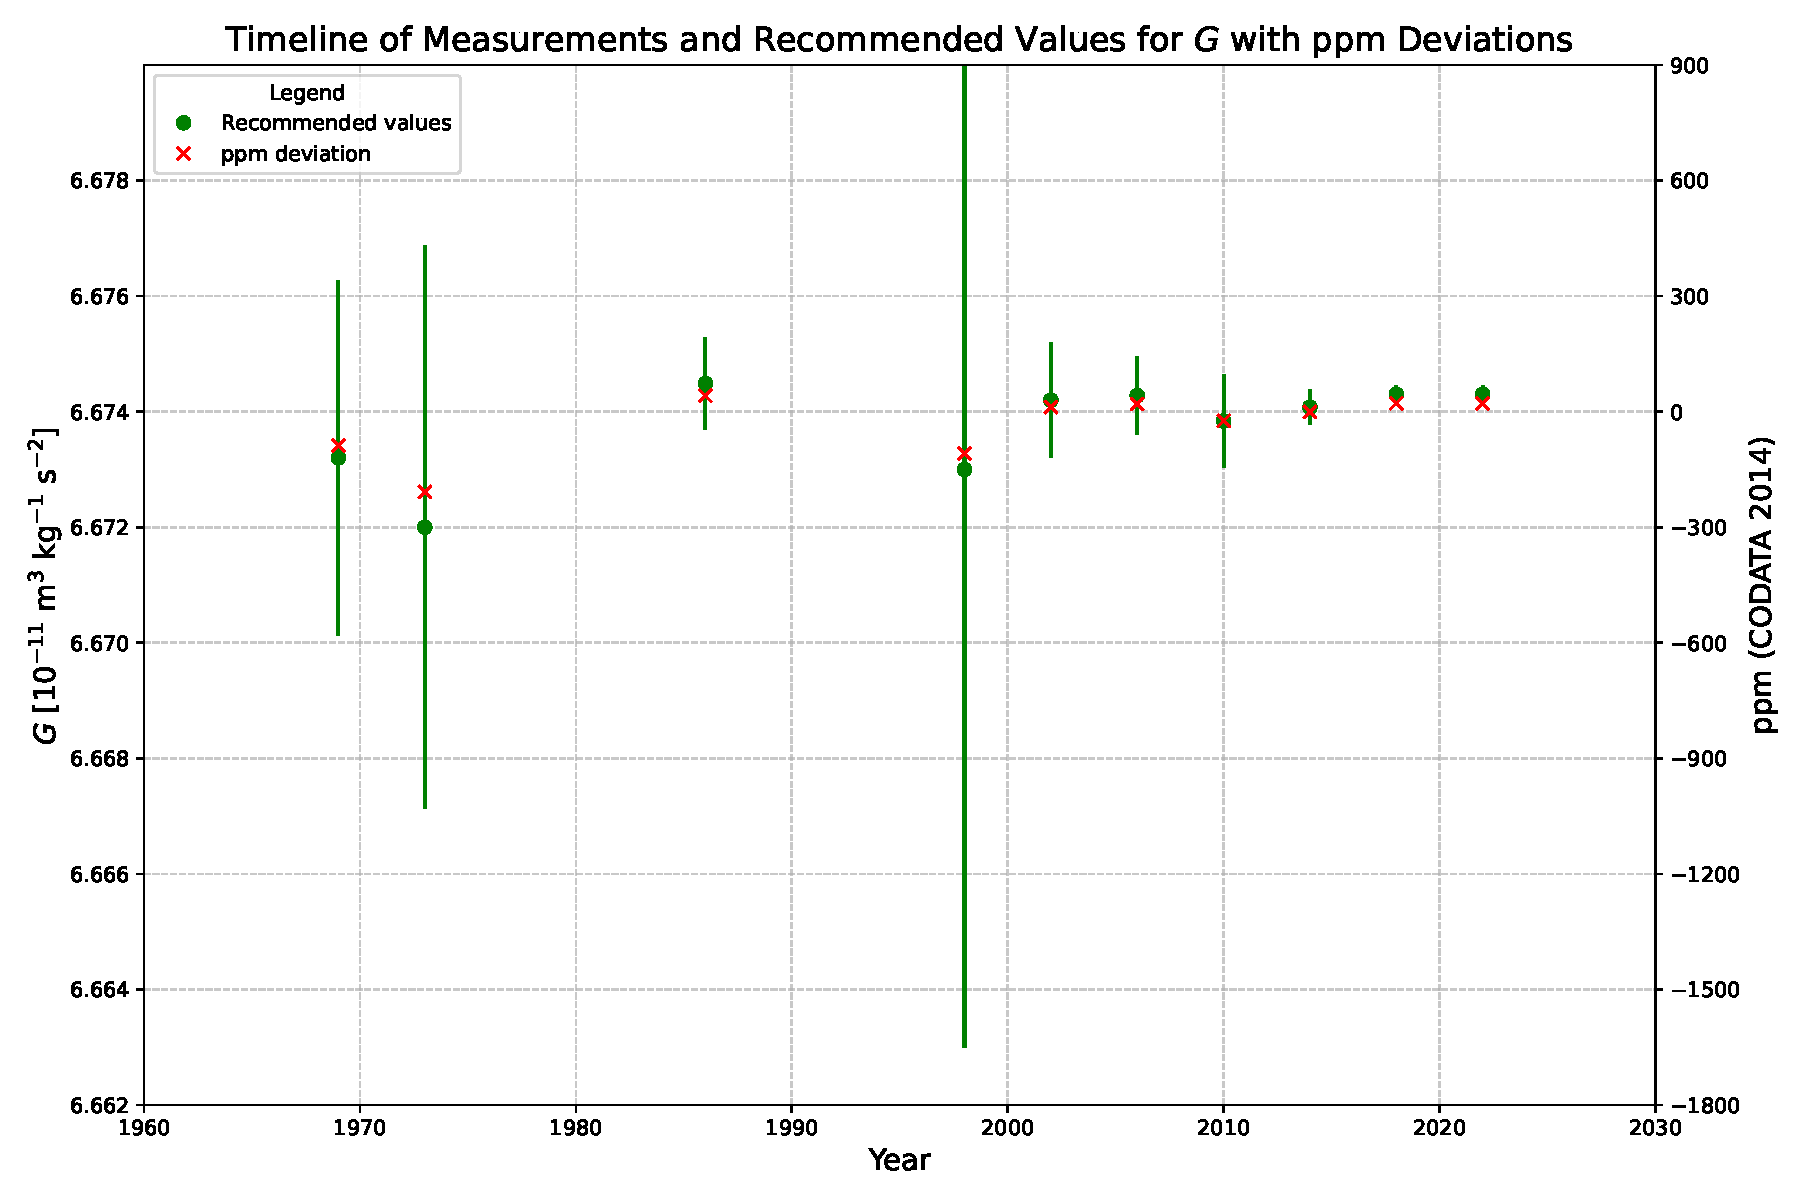
\includegraphics[width=0.8\textwidth]{Visualizations/gravitational_constant.pdf} % Replace with your file name
    \caption{Measures history of Gravitational Constant G, Source \cite{wikipedia2025gconst}}
    \label{fig:G}
\end{figure}

\subsection{My Favourite Tools}
My favourite tool for creating data visualizations is surely ChatGPT. It helps in the creation of a visualization from A to Z: data cleaning, data interpretation, data plotting and everything feels easier and faster. Quick visualization of an idea helps a lot in the evaluation of the quality of a chart from the beginning, discarding inappropriate type of charts. When the sketch begins to take life, it is straightforward to modify it in order to have a visualization with a personal touch. Clearly the Python language has a role in the simplification of the process, the python packages for data visualization offer a huge variety of charts and plots and are easy to familiarize with.
My favourite sources for datasets are the US Government web sites, there is nothing better to ask for: user-friendly, rich in content (data and plot examples) and completely free. The fact that the US makes this amount of scientific/ economic data free of use is incredible. An honorable mention to the NASA website, which is on Google Chrome Bookmark list from now on. Last but not least, \href{netlify.com}{netlify.com}, the provider where I deployed my interactive visualization through GitHub: simple, fast and reliable... My only regret is to not have a complete interactive portfolio.

\section{Bibliography}
\bibliographystyle{abbrv}
\bibliography{references}
\subsection{Data Sources}

\subsection{Software and Tools Used}
% [List all tools, packages, and software used.]
Python Packages
\begin{itemize}
    \item matplotlib, numpy, pandas, plotly, dash, os, subprocess
\end{itemize}
Software
\begin{itemize}
    \item Visual Studio Code, GPT-4o, My GPTs, netlify.com
\end{itemize}

\subsection{Generative AI Disclosure}
As part of the objectives of this portfolio, for every visualization, with the exception of figure \ref{fig:bad} and \ref{fig:good}, generative AI tools such as ChatGPT have been utilized to assist in their creation. All AI-generated outputs were reviewed and finalized by the author to ensure accuracy and alignment with the intended goals. 


\section{Appendix}
\textbf{Screenshots of AI Conversations:}
\begin{figure}[H]
    \centering
    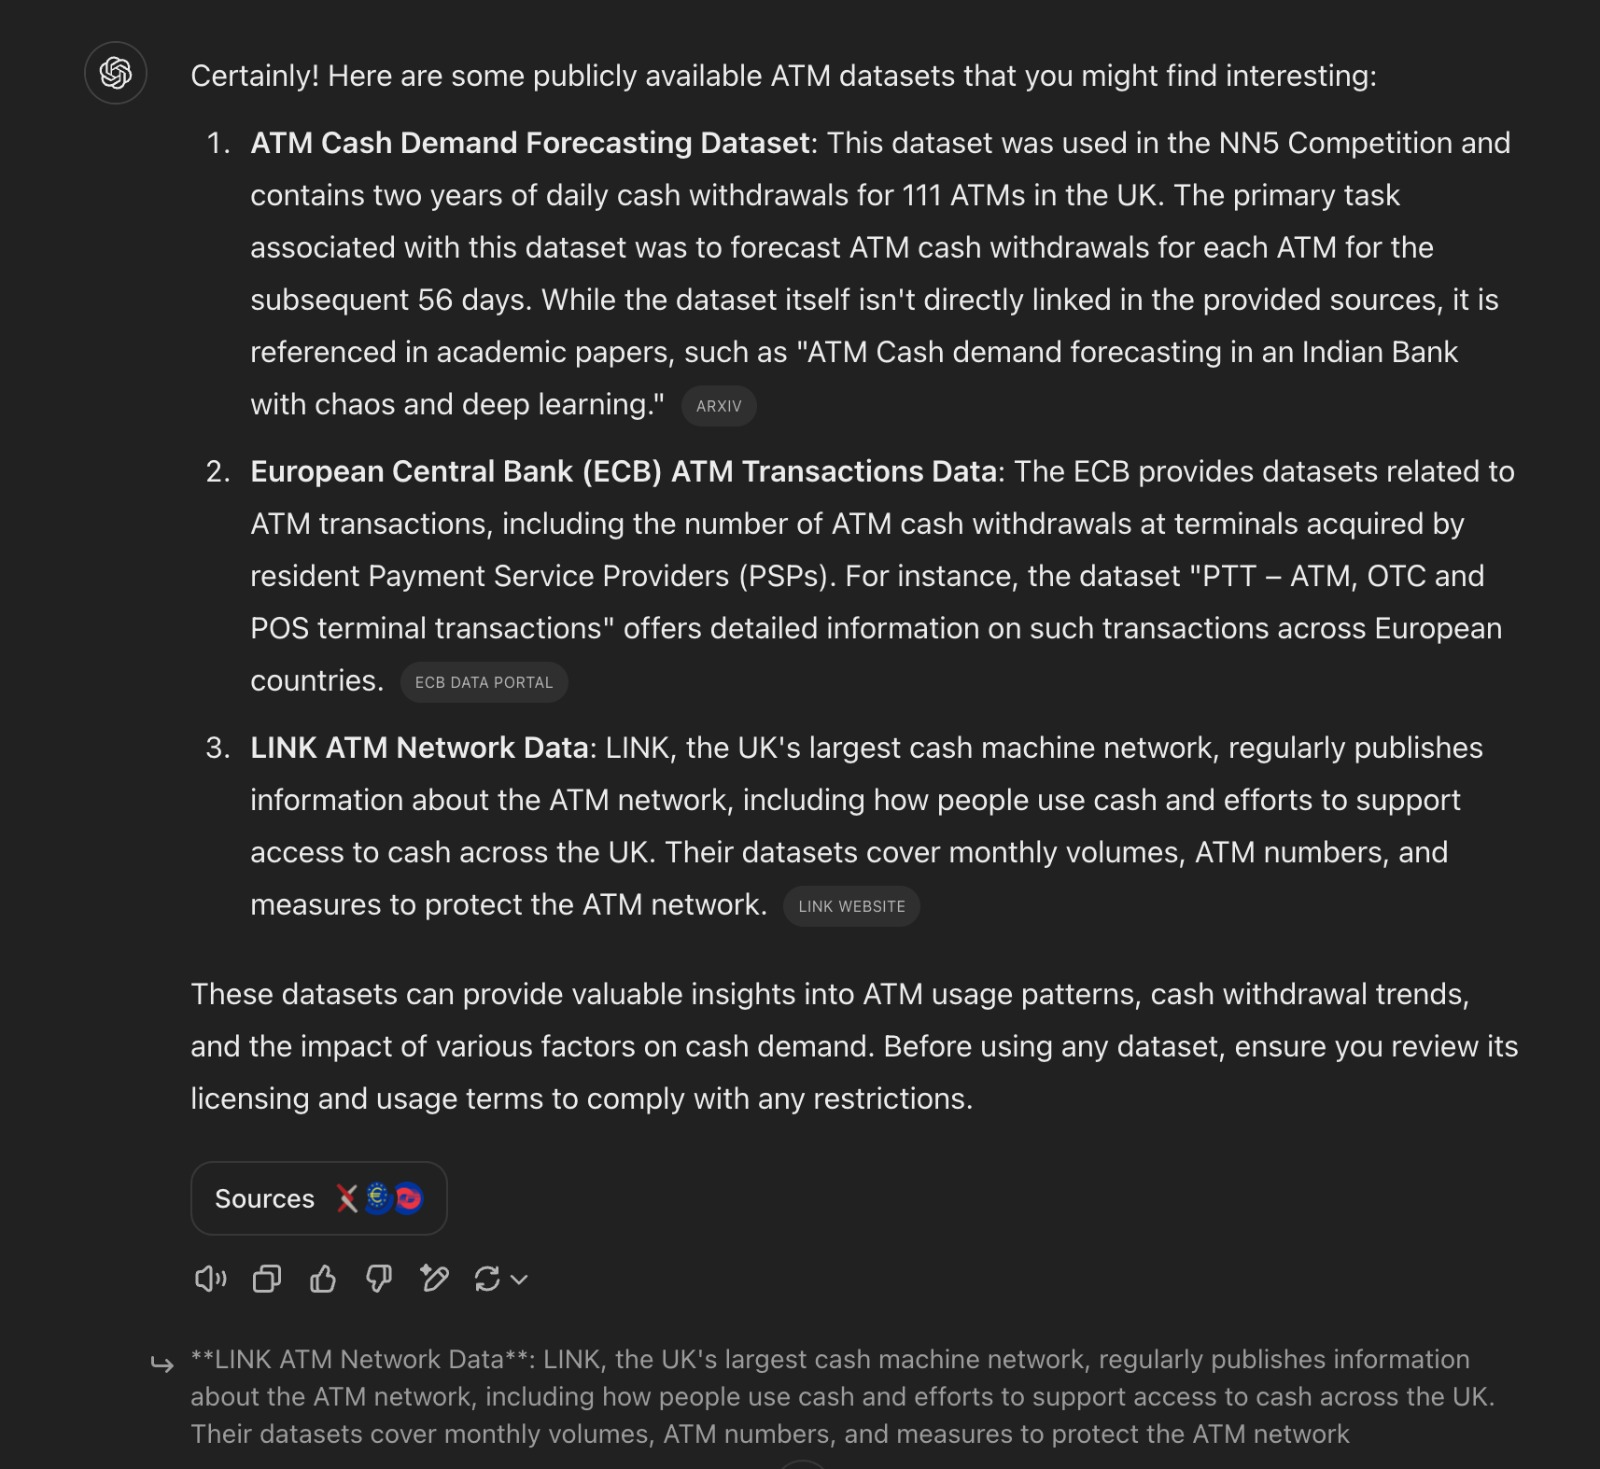
\includegraphics[width=0.8\textwidth]{WhatsApp Image 2025-01-17 at 20.09.52.jpeg} % Replace with your file name
    \caption{}
    \label{fig:}
\end{figure}
\begin{figure}[H]
    \centering
    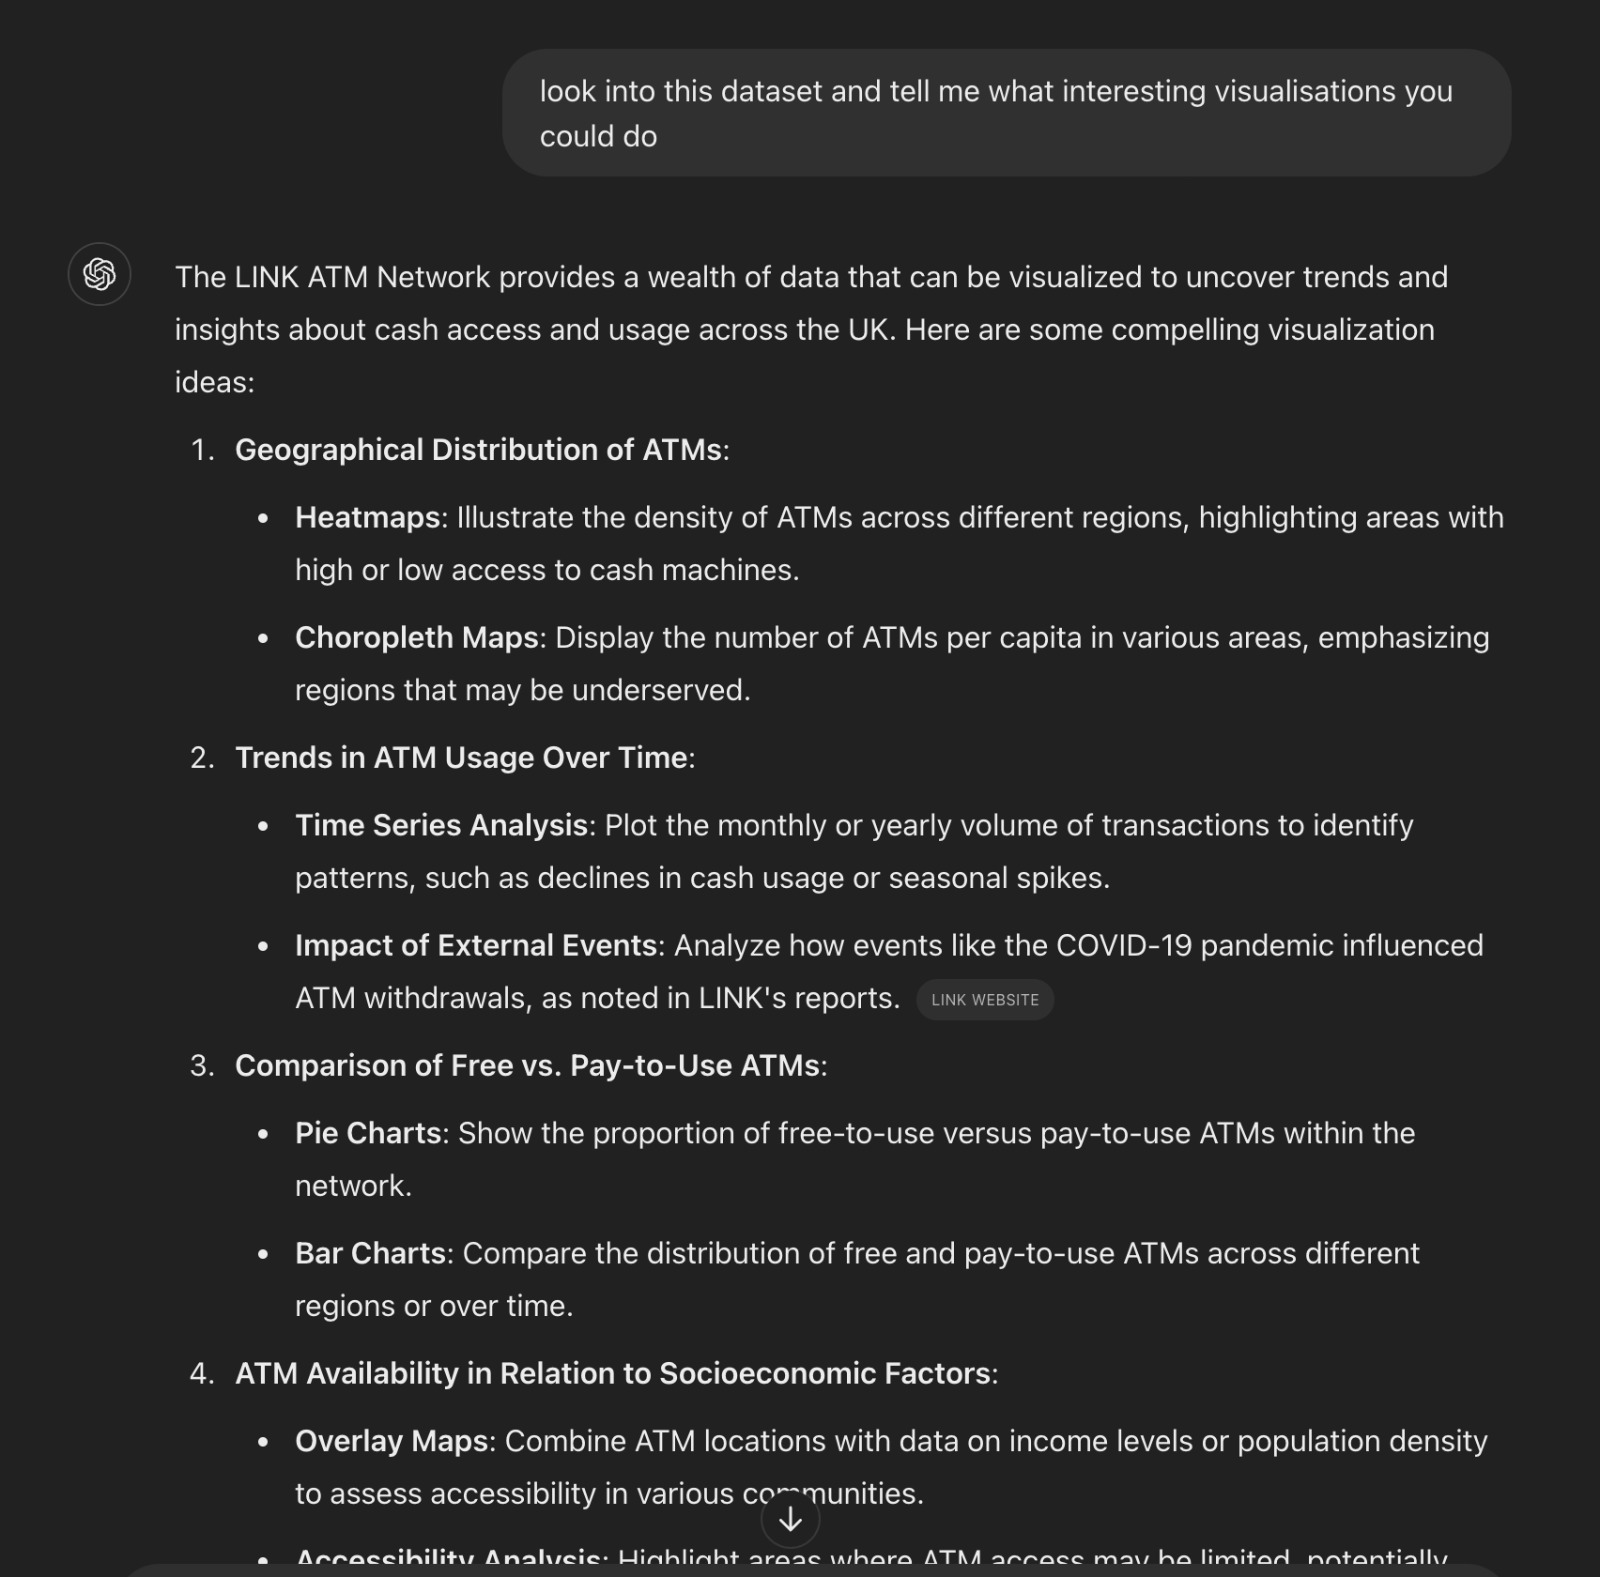
\includegraphics[width=0.8\textwidth]{WhatsApp Image 2025-01-17 at 20.10.09.jpeg} % Replace with your file name
    \caption{}
    \label{fig:}
\end{figure}
\begin{figure}[H]
    \centering
    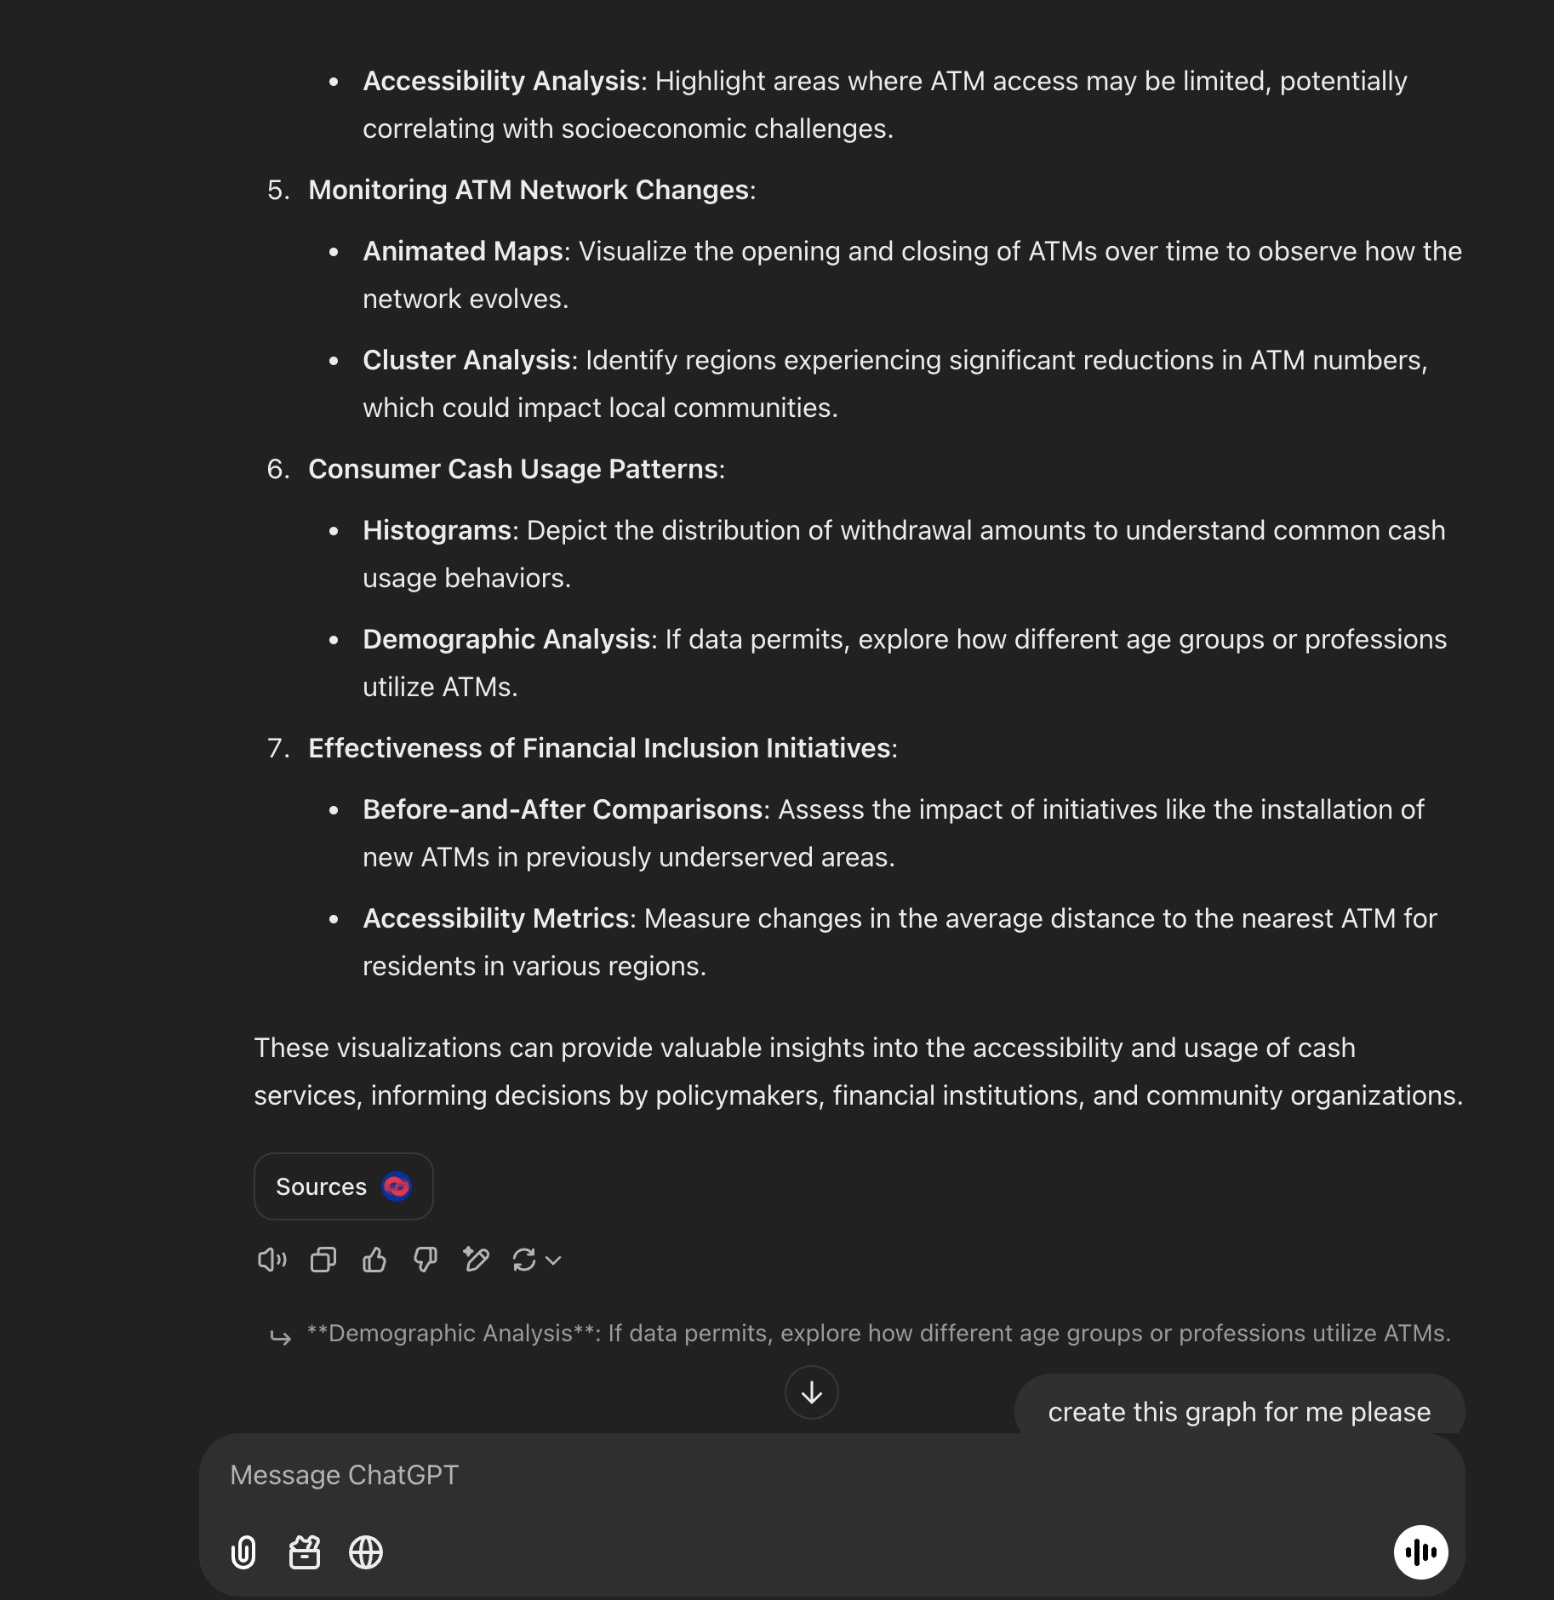
\includegraphics[width=0.8\textwidth]{WhatsApp Image 2025-01-17 at 20.10.28.jpeg} % Replace with your file name
    \caption{}
    \label{fig:}
\end{figure}
\begin{figure}[H]
    \centering
    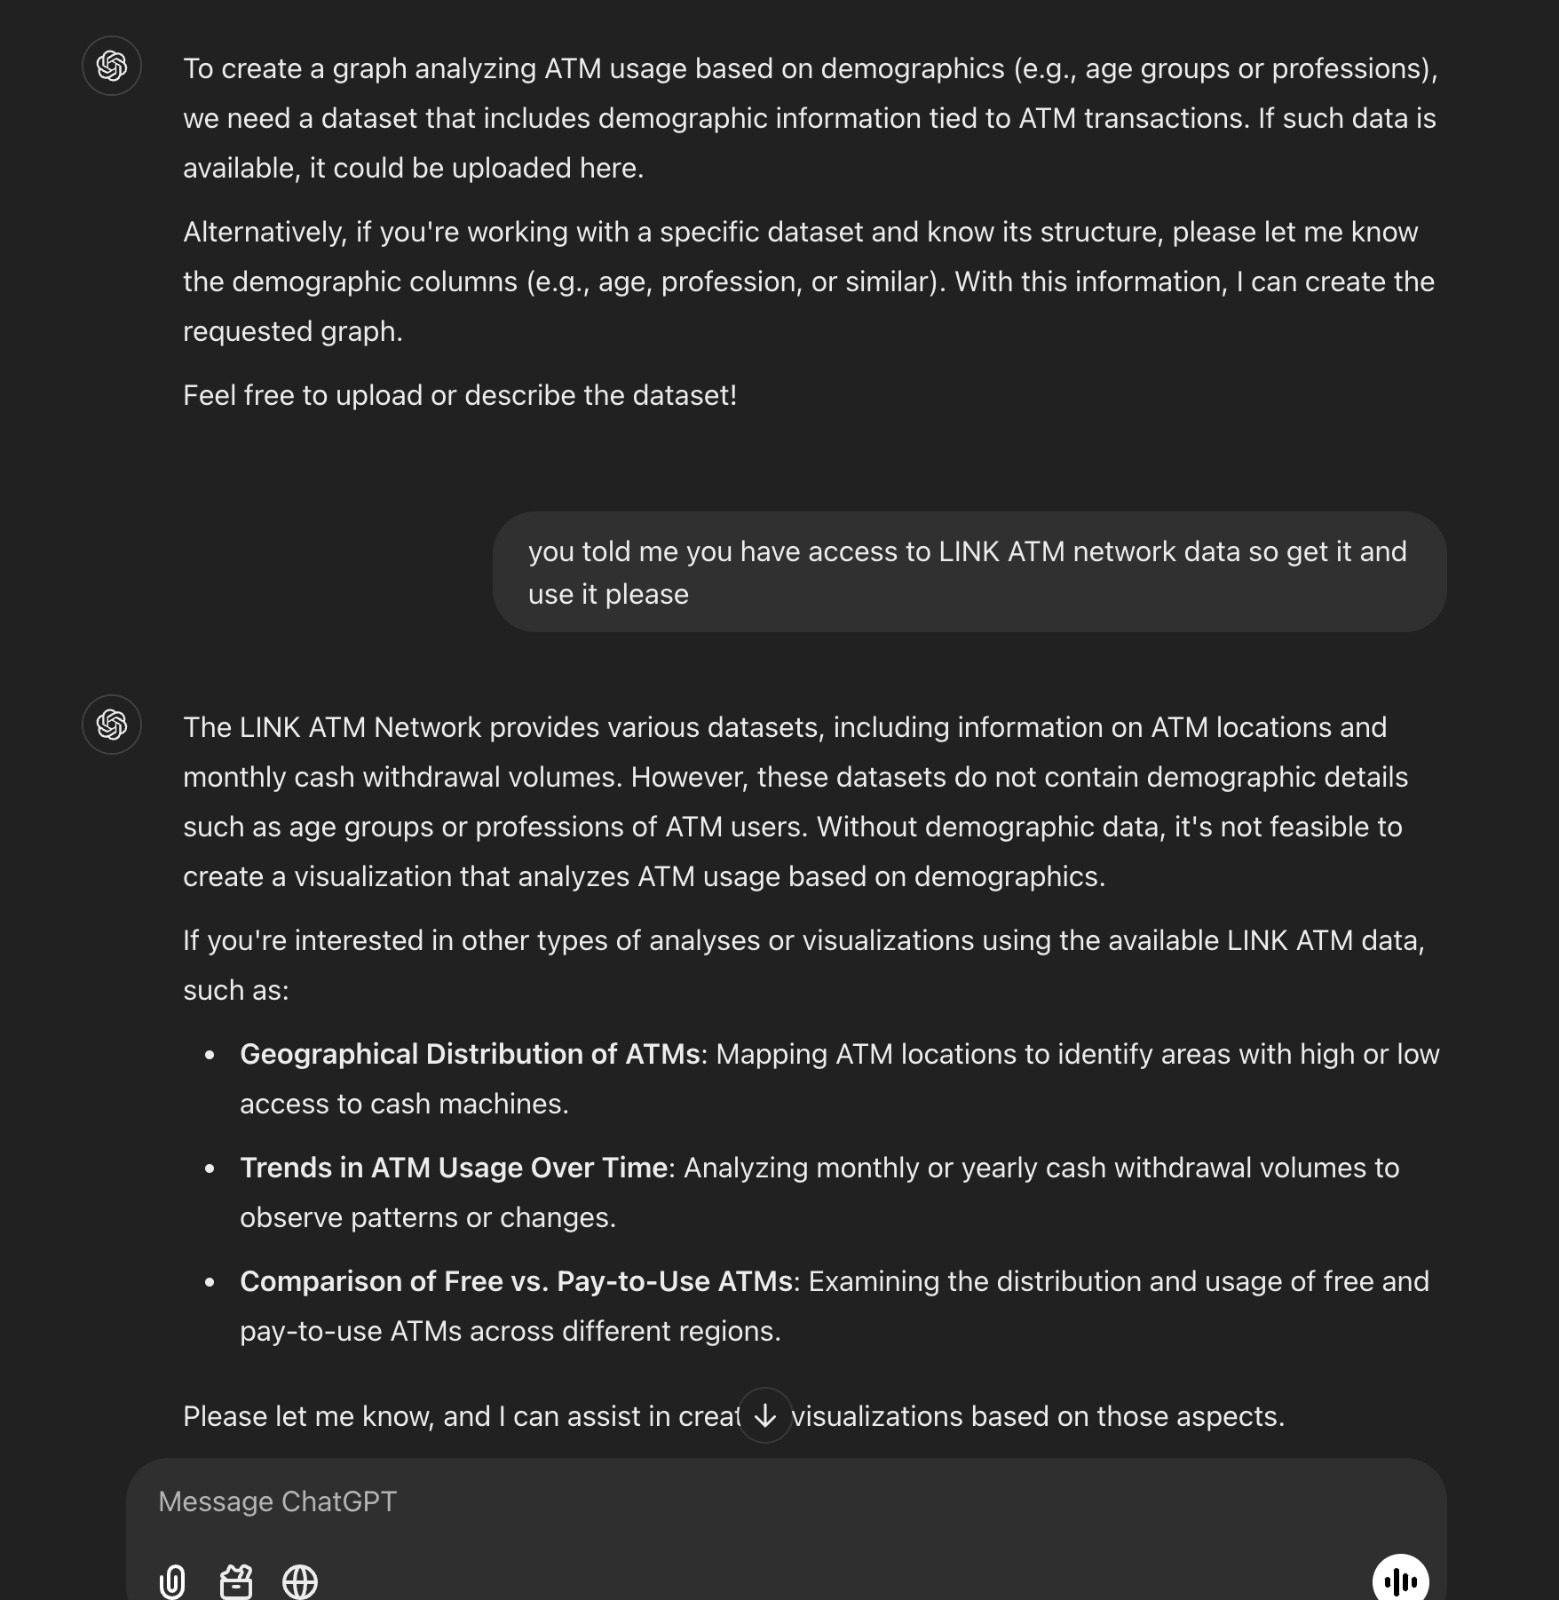
\includegraphics[width=0.8\textwidth]{WhatsApp Image 2025-01-17 at 20.10.43.jpeg} % Replace with your file name
    \caption{}
    \label{fig:}
\end{figure}
\begin{figure}[H]
    \centering
    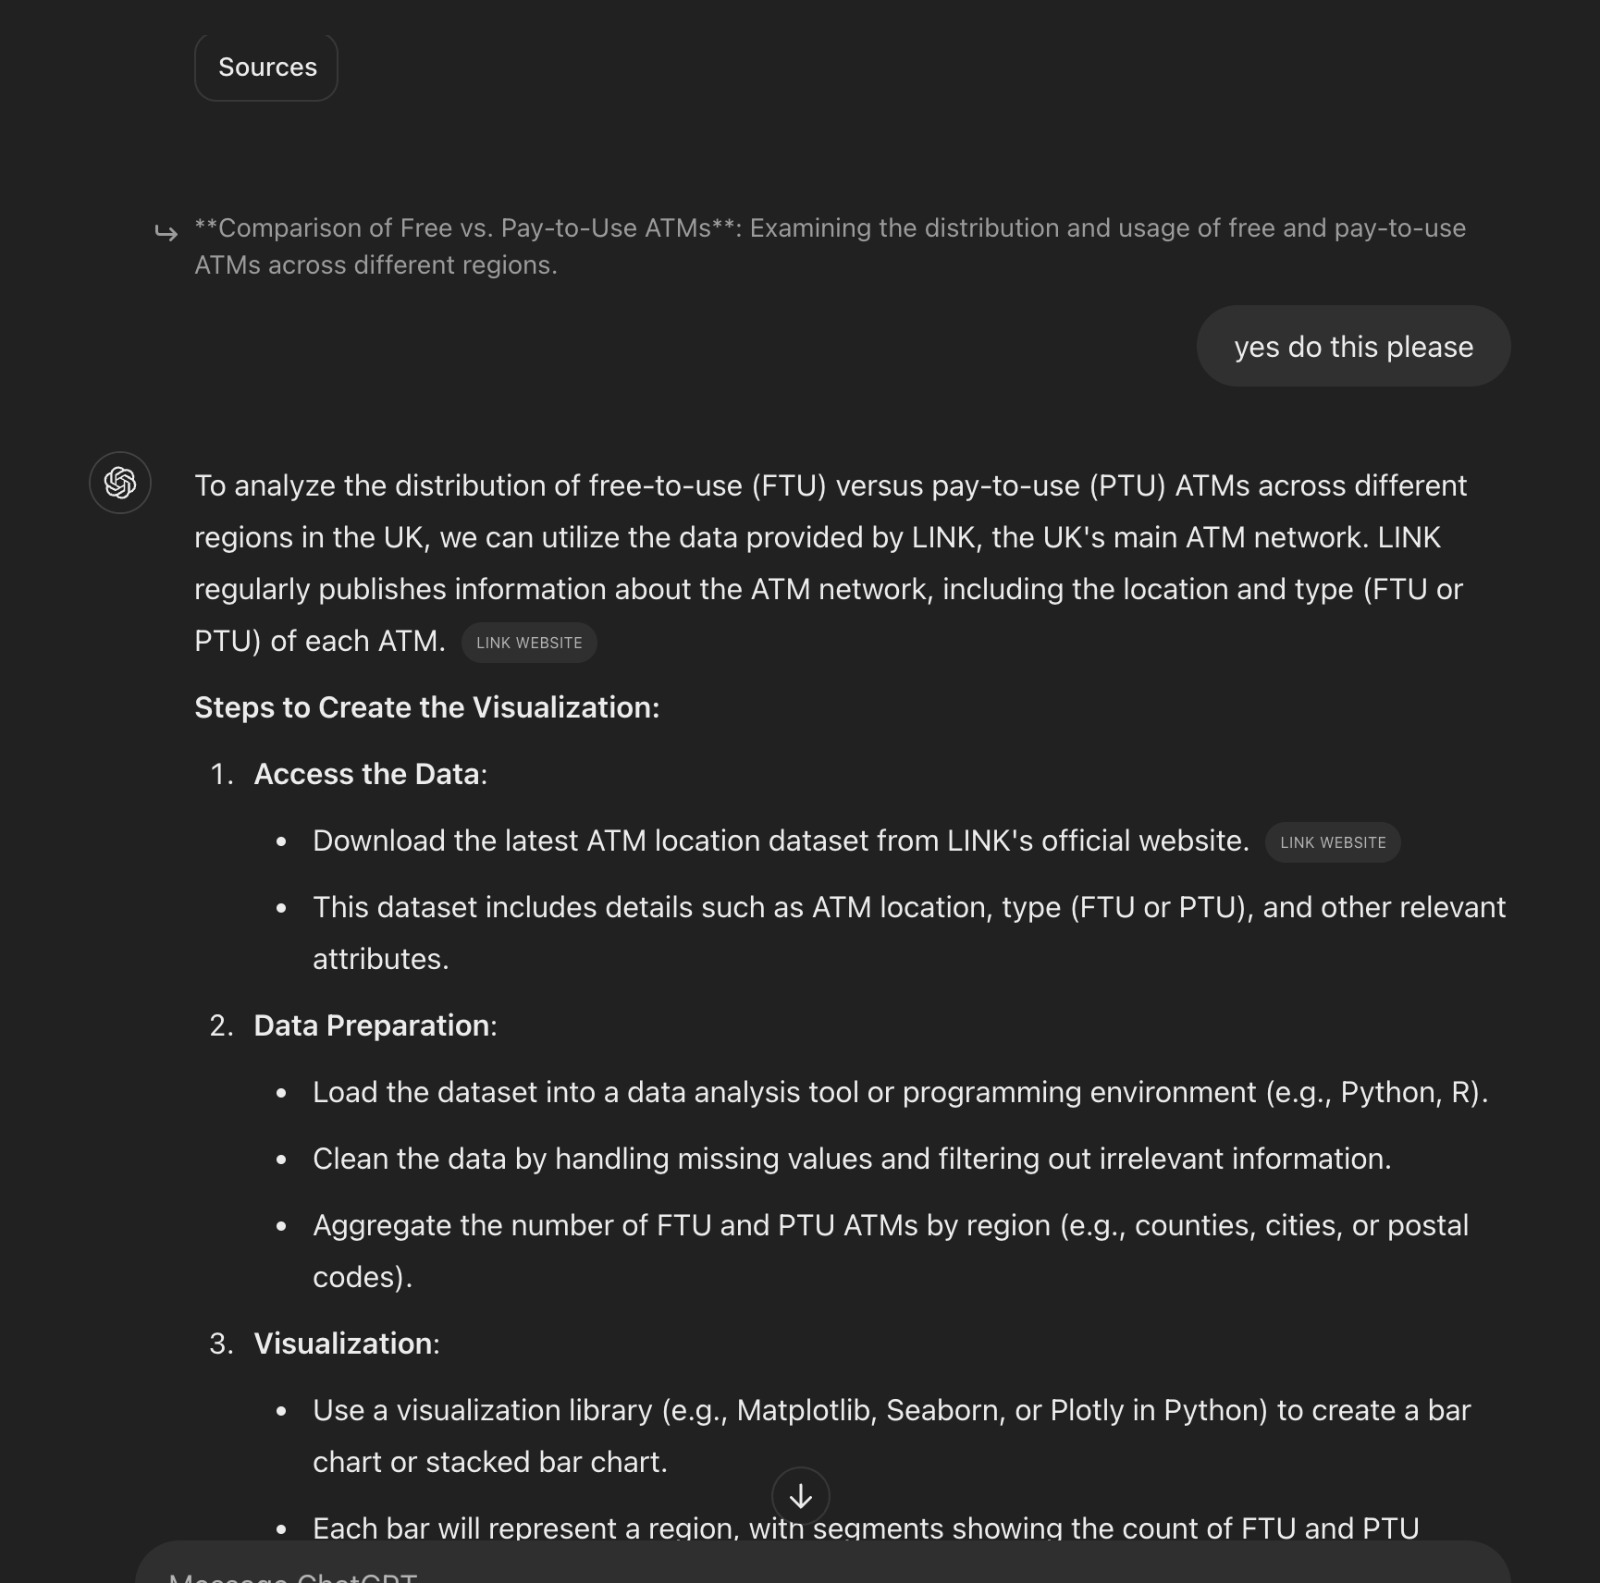
\includegraphics[width=0.8\textwidth]{WhatsApp Image 2025-01-17 at 20.10.59.jpeg} % Replace with your file name
    \caption{}
    \label{fig:}
\end{figure}
\begin{figure}[H]
    \centering
    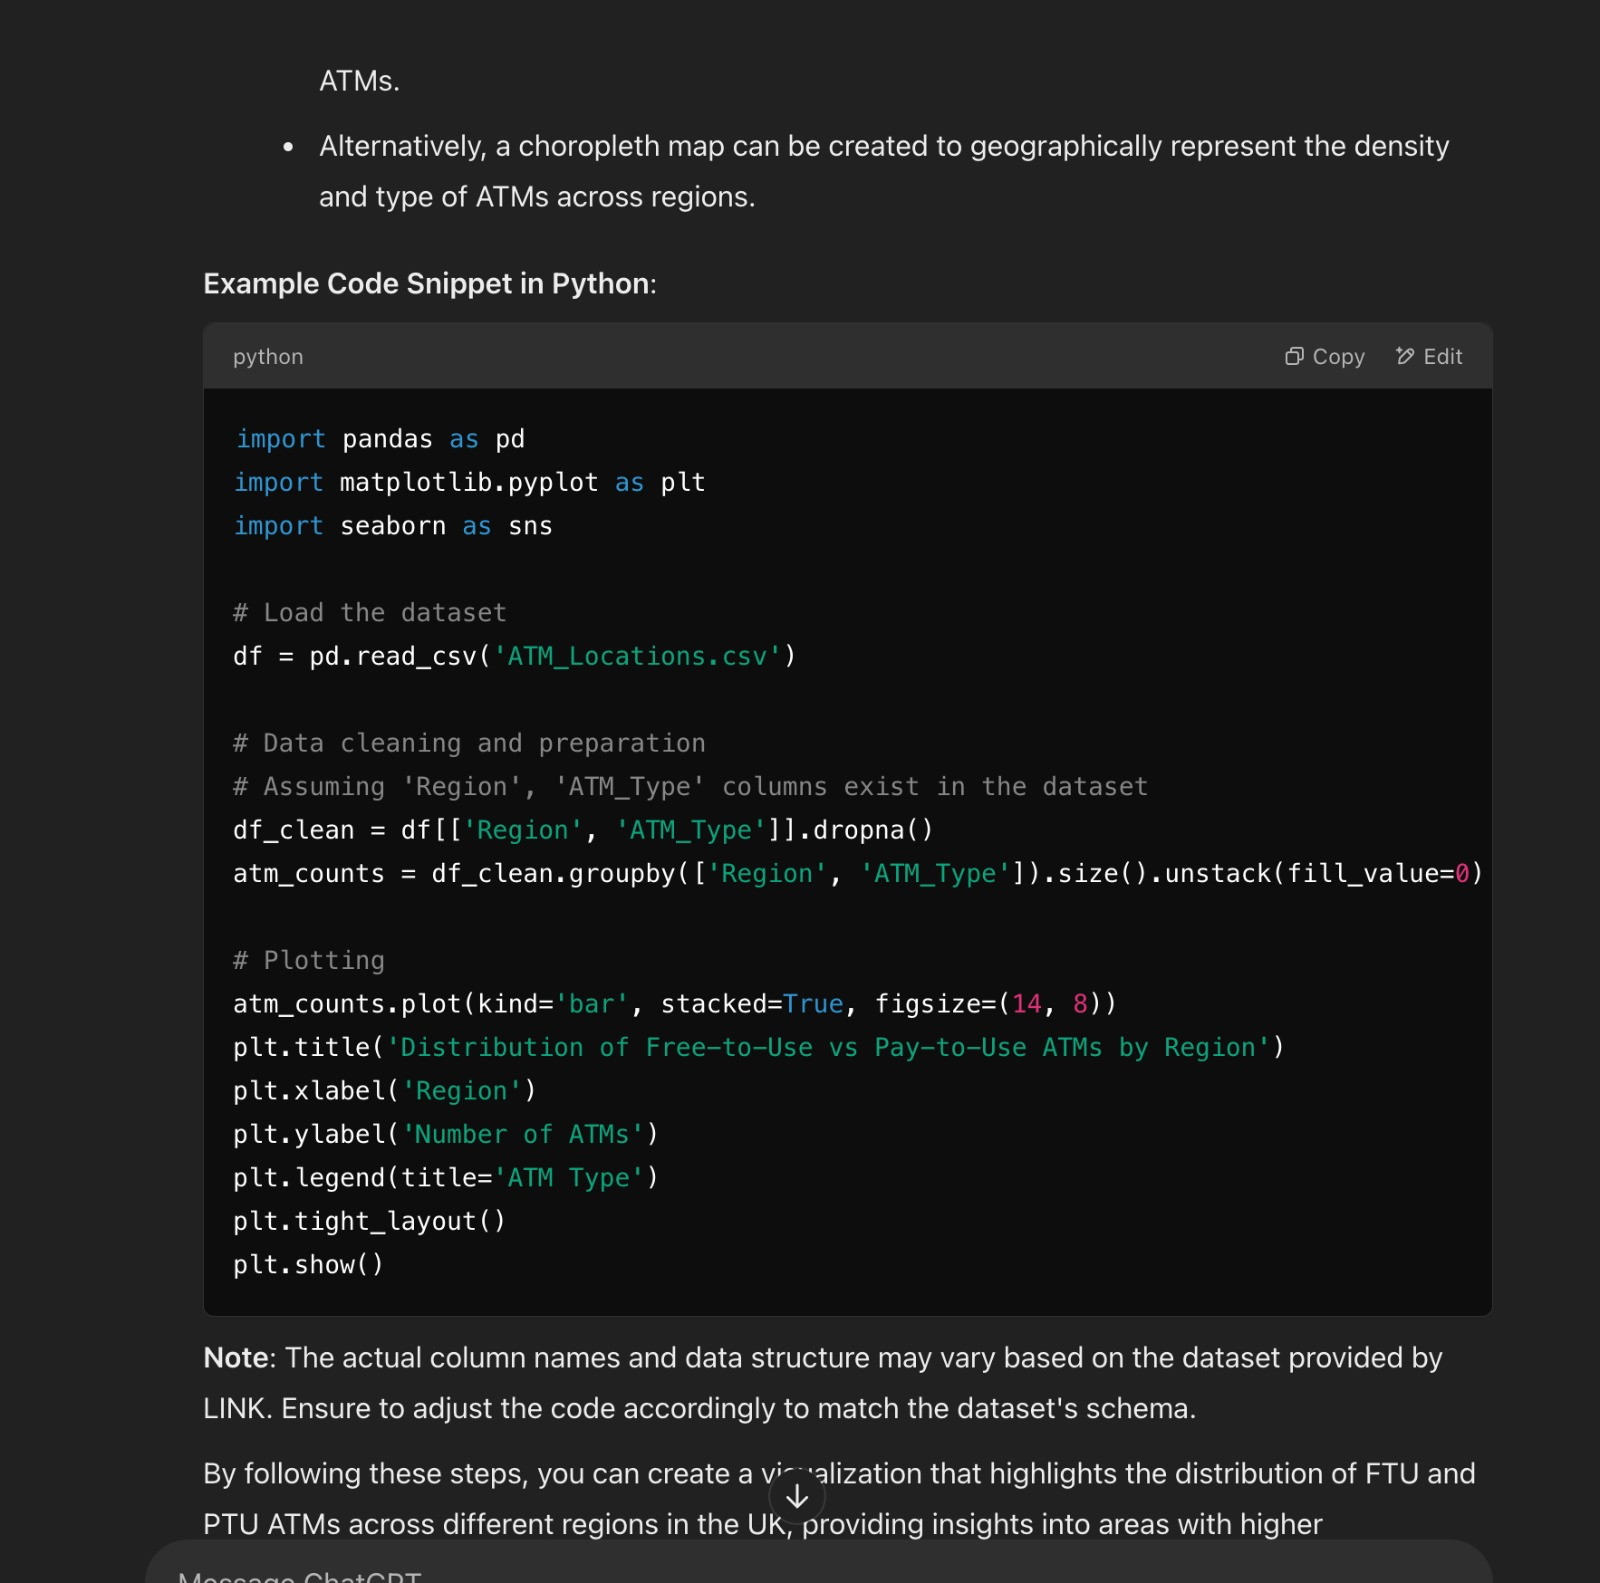
\includegraphics[width=0.8\textwidth]{WhatsApp Image 2025-01-17 at 20.11.13.jpeg} % Replace with your file name
    \caption{}
    \label{fig:}
\end{figure}
\begin{figure}[H]
    \centering
    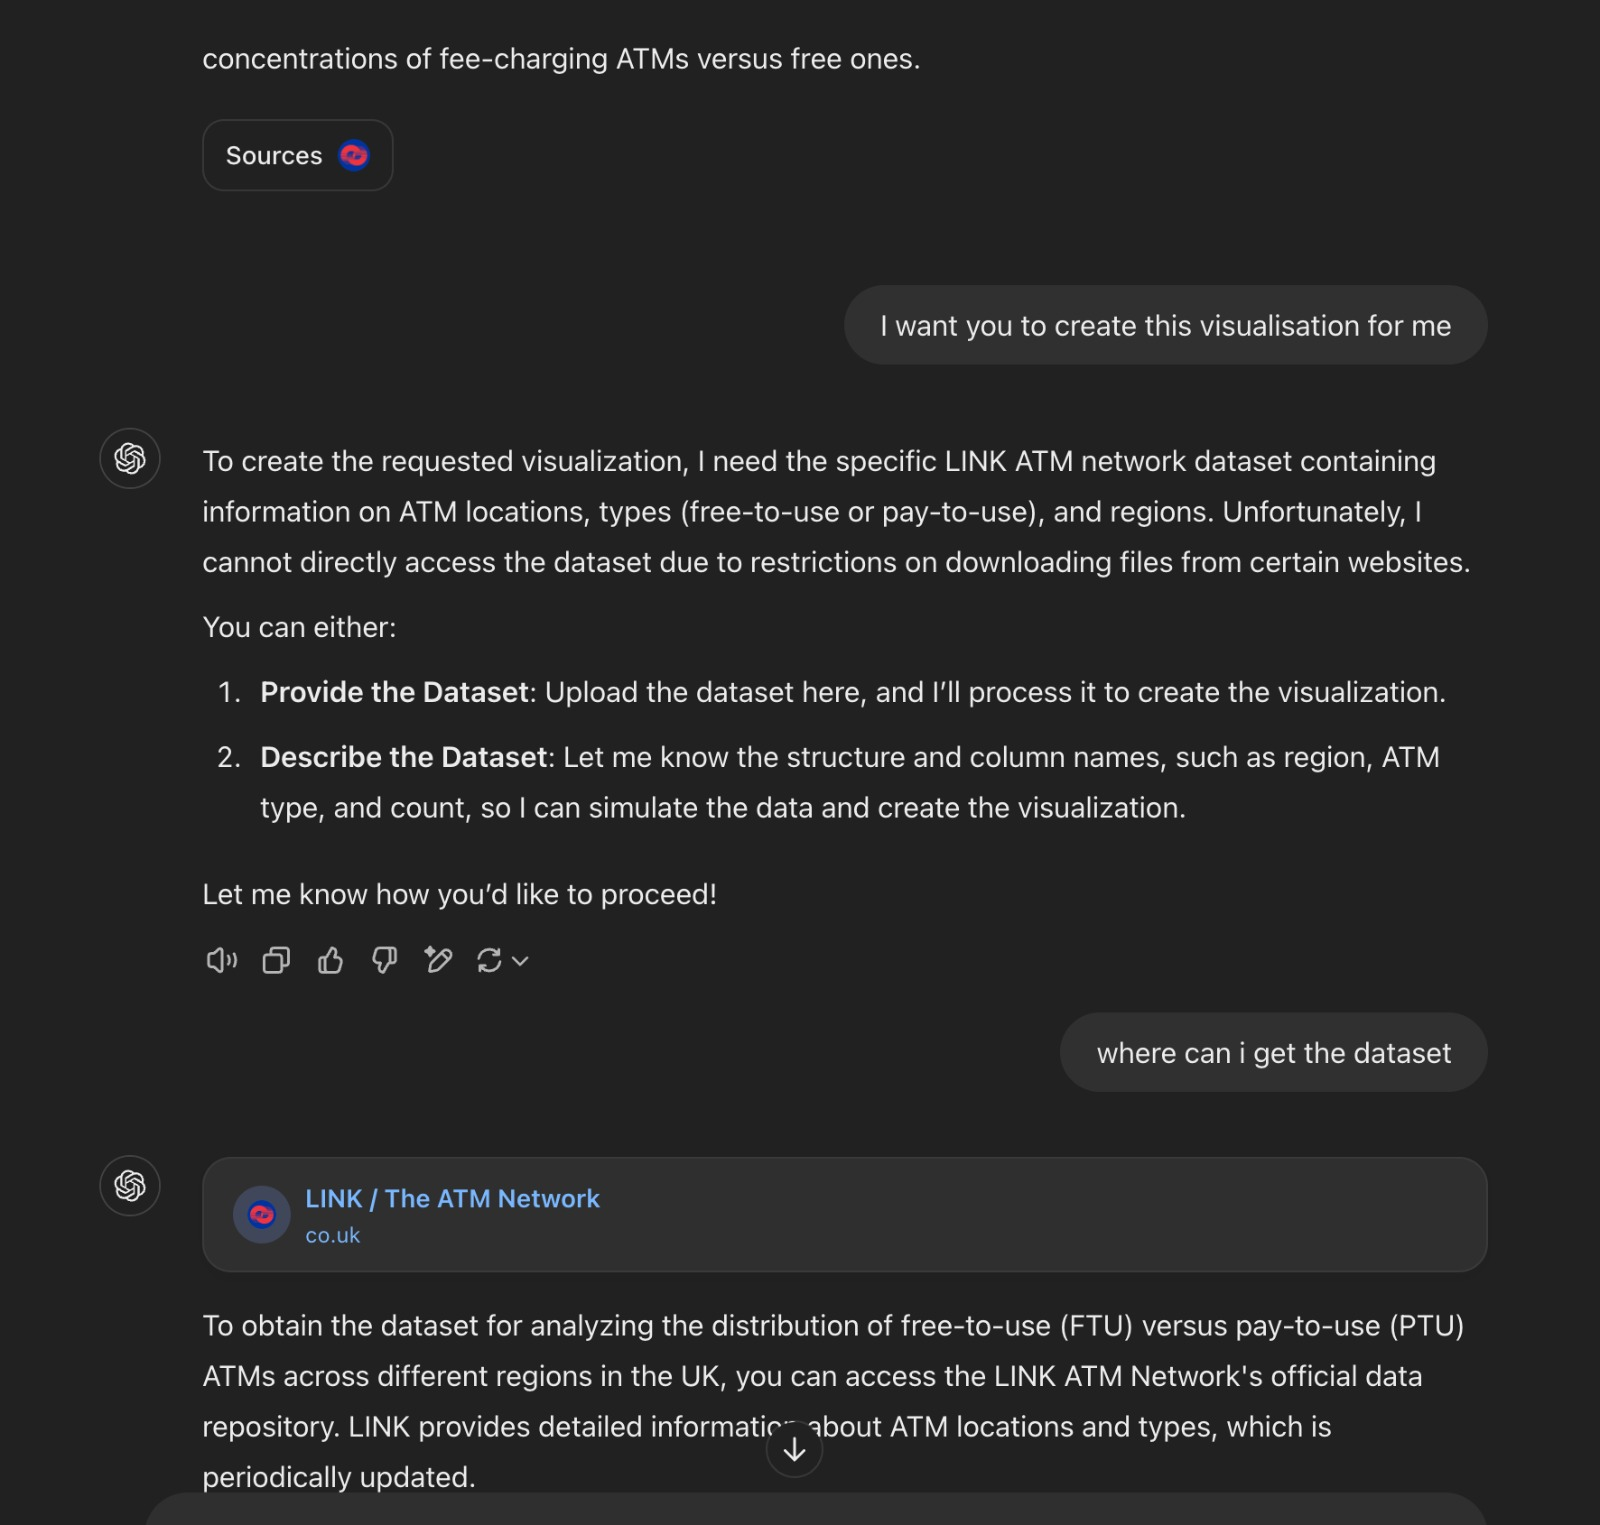
\includegraphics[width=0.8\textwidth]{WhatsApp Image 2025-01-17 at 20.11.27.jpeg} % Replace with your file name
    \caption{}
    \label{fig:}
\end{figure}
\begin{figure}[H]
    \centering
    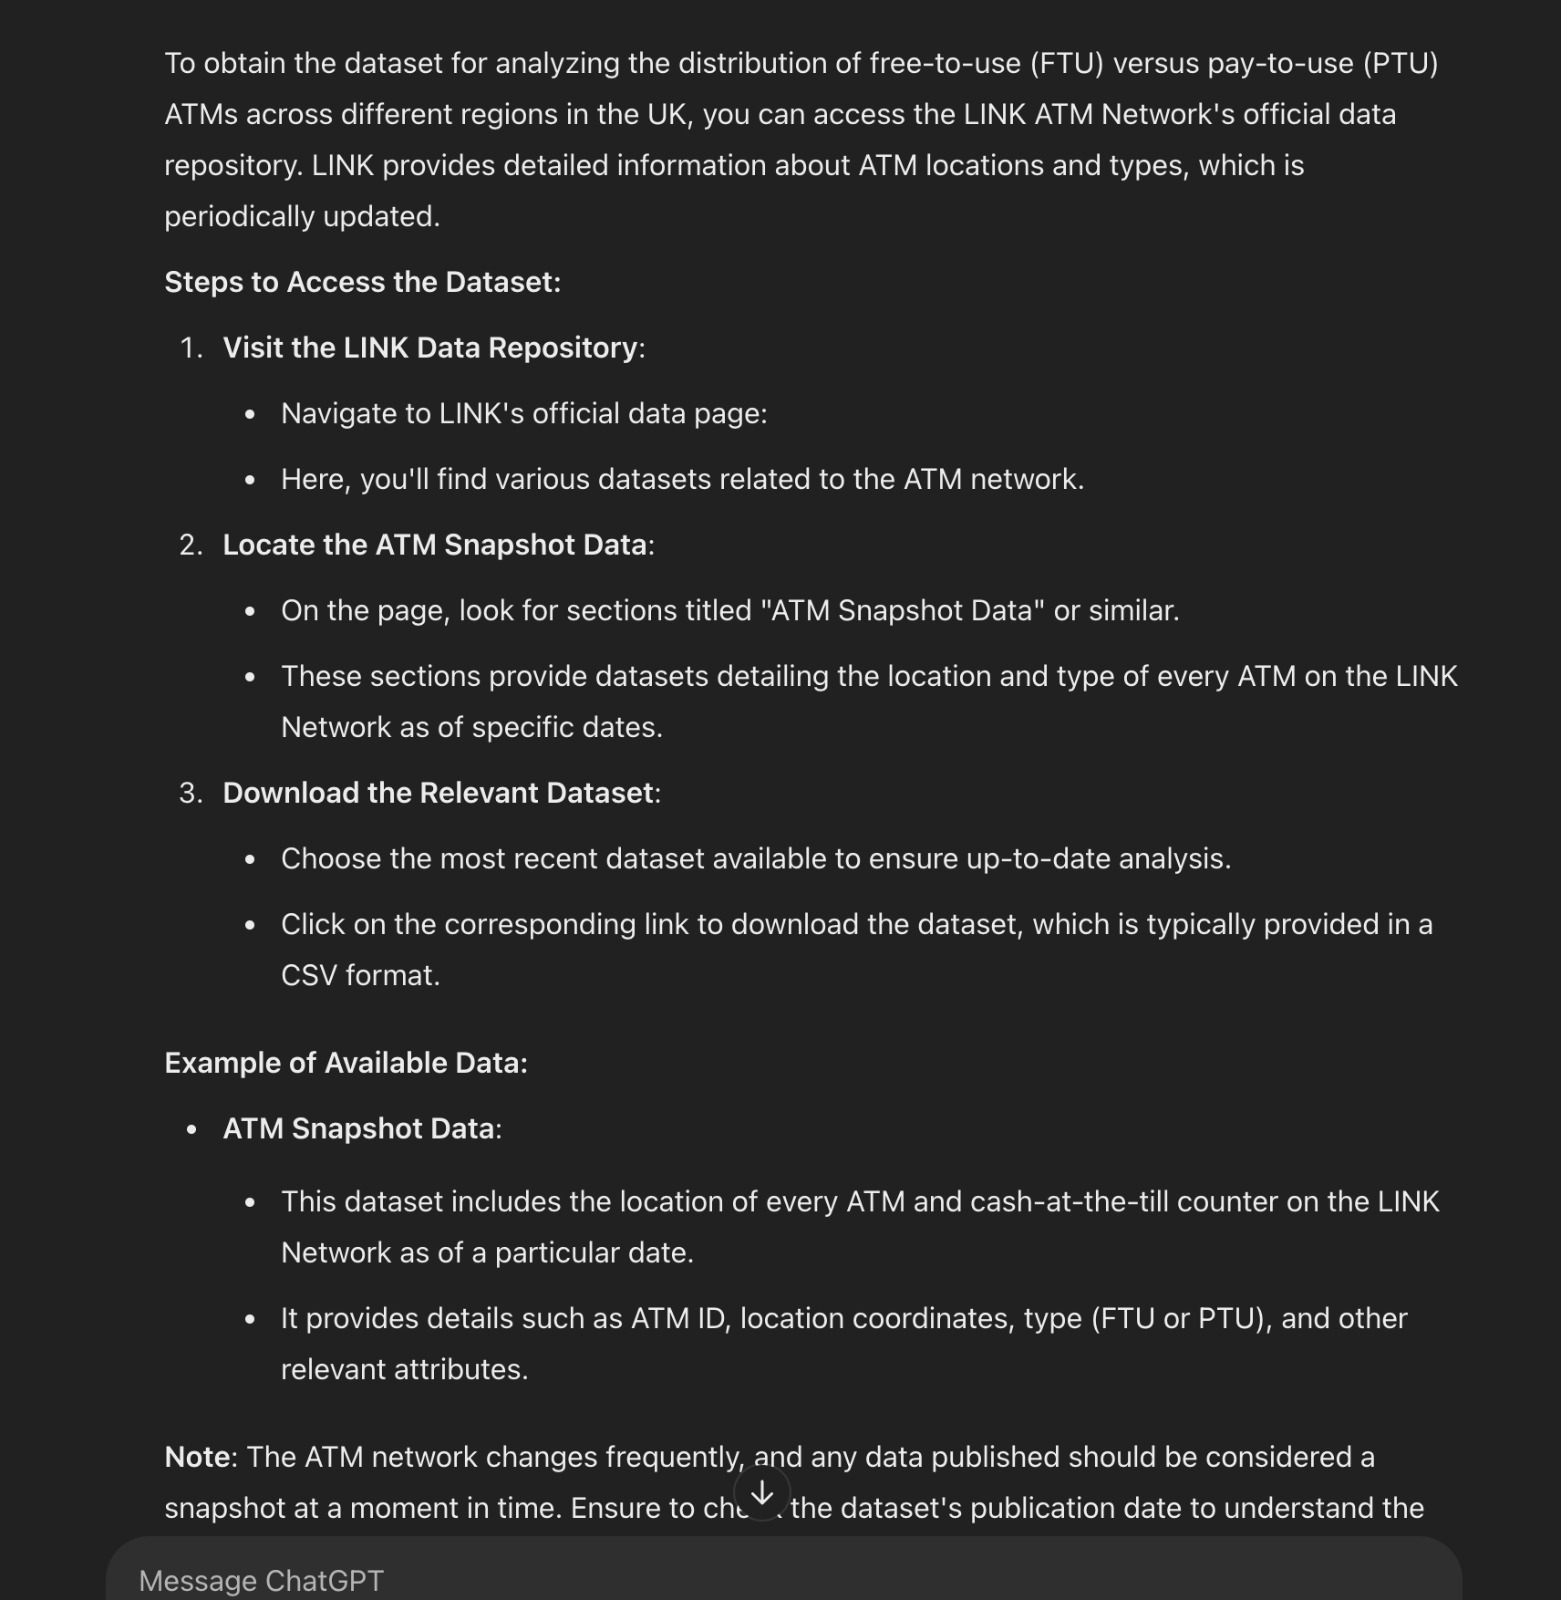
\includegraphics[width=0.8\textwidth]{WhatsApp Image 2025-01-17 at 20.11.40.jpeg} % Replace with your file name
    \caption{}
    \label{fig:}
\end{figure}
\begin{figure}[H]
    \centering
    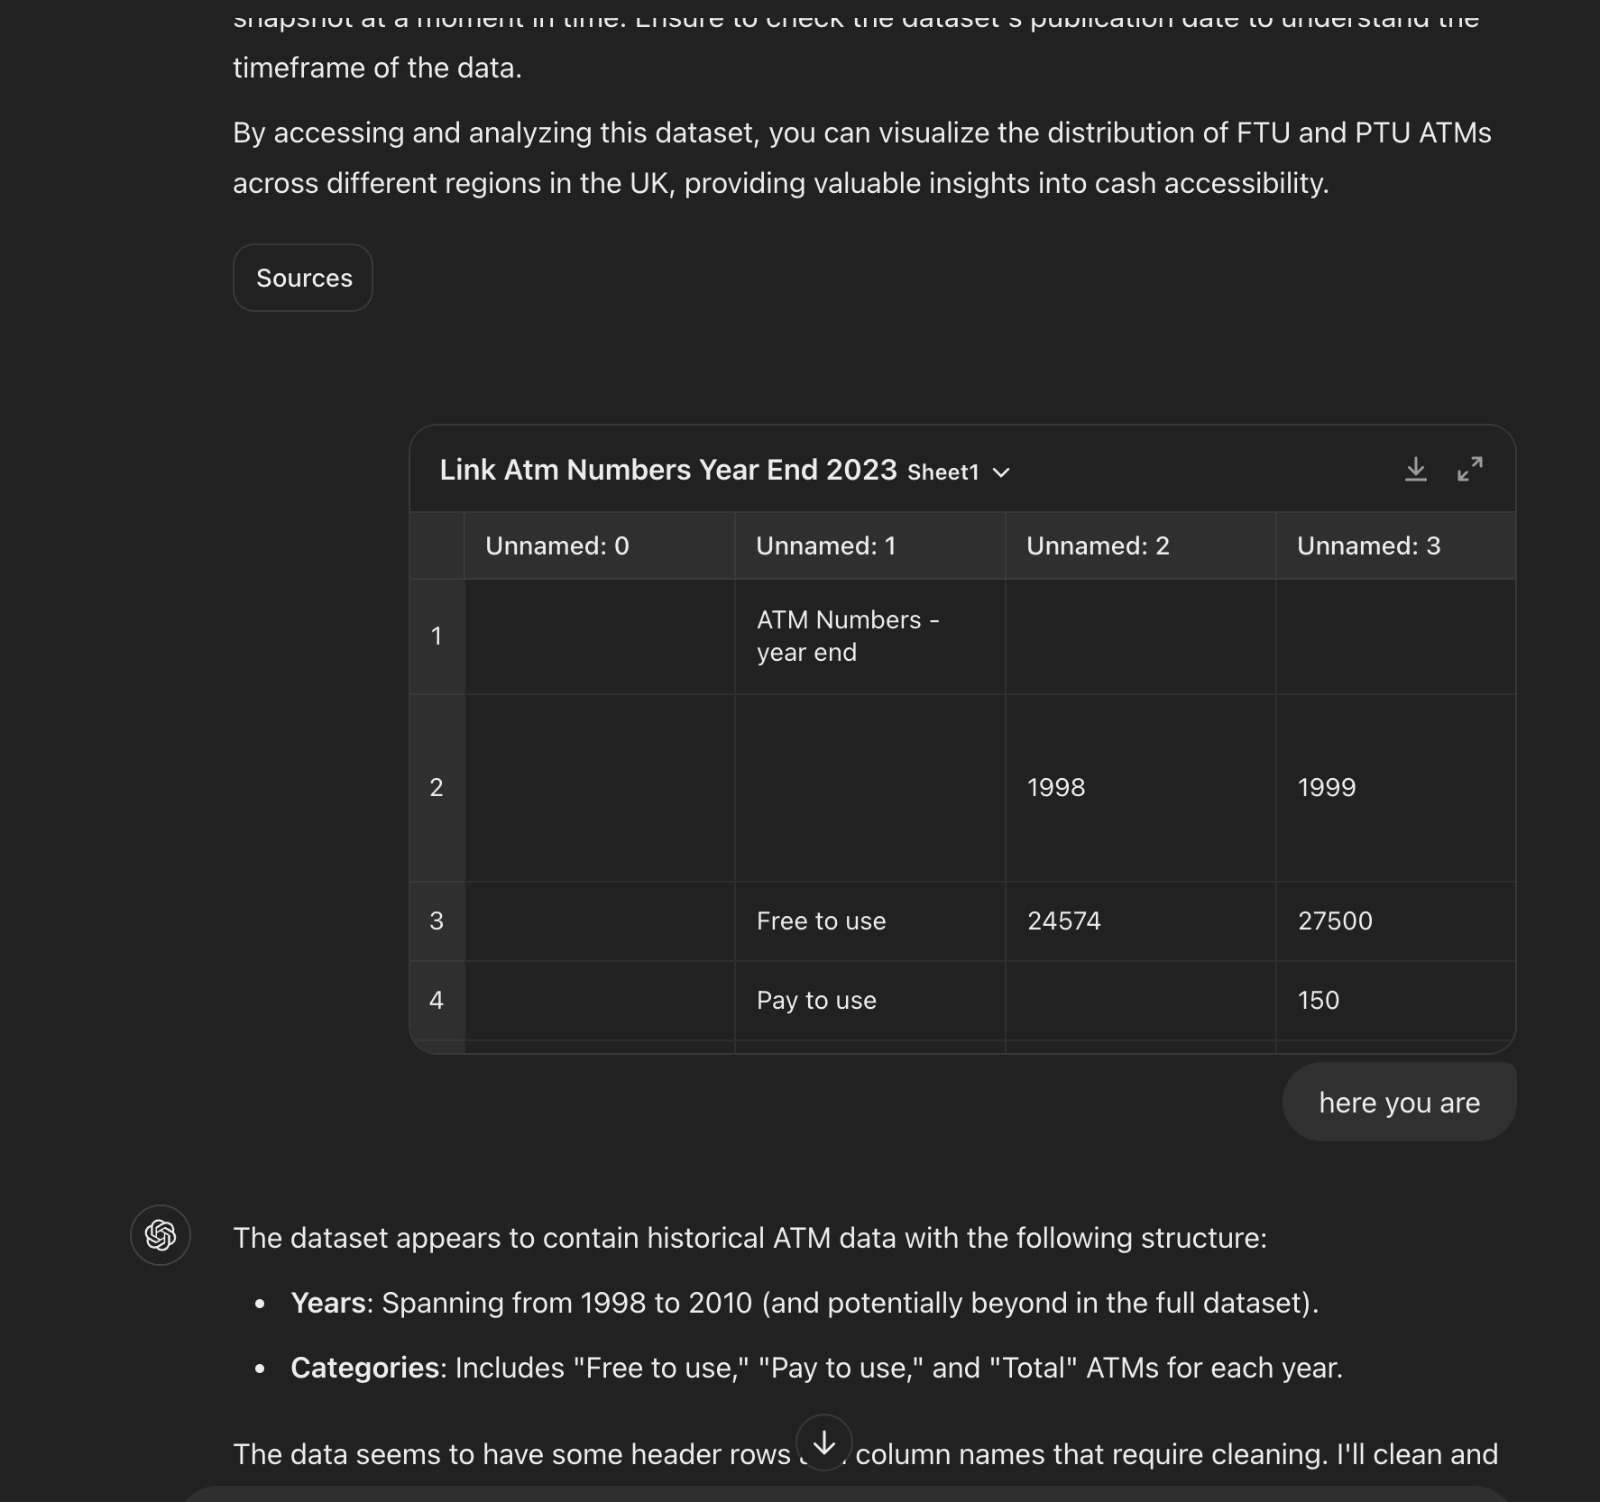
\includegraphics[width=0.8\textwidth]{WhatsApp Image 2025-01-17 at 20.11.54.jpeg} % Replace with your file name
    \caption{}
    \label{fig:}
\end{figure}
\begin{figure}[H]
    \centering
    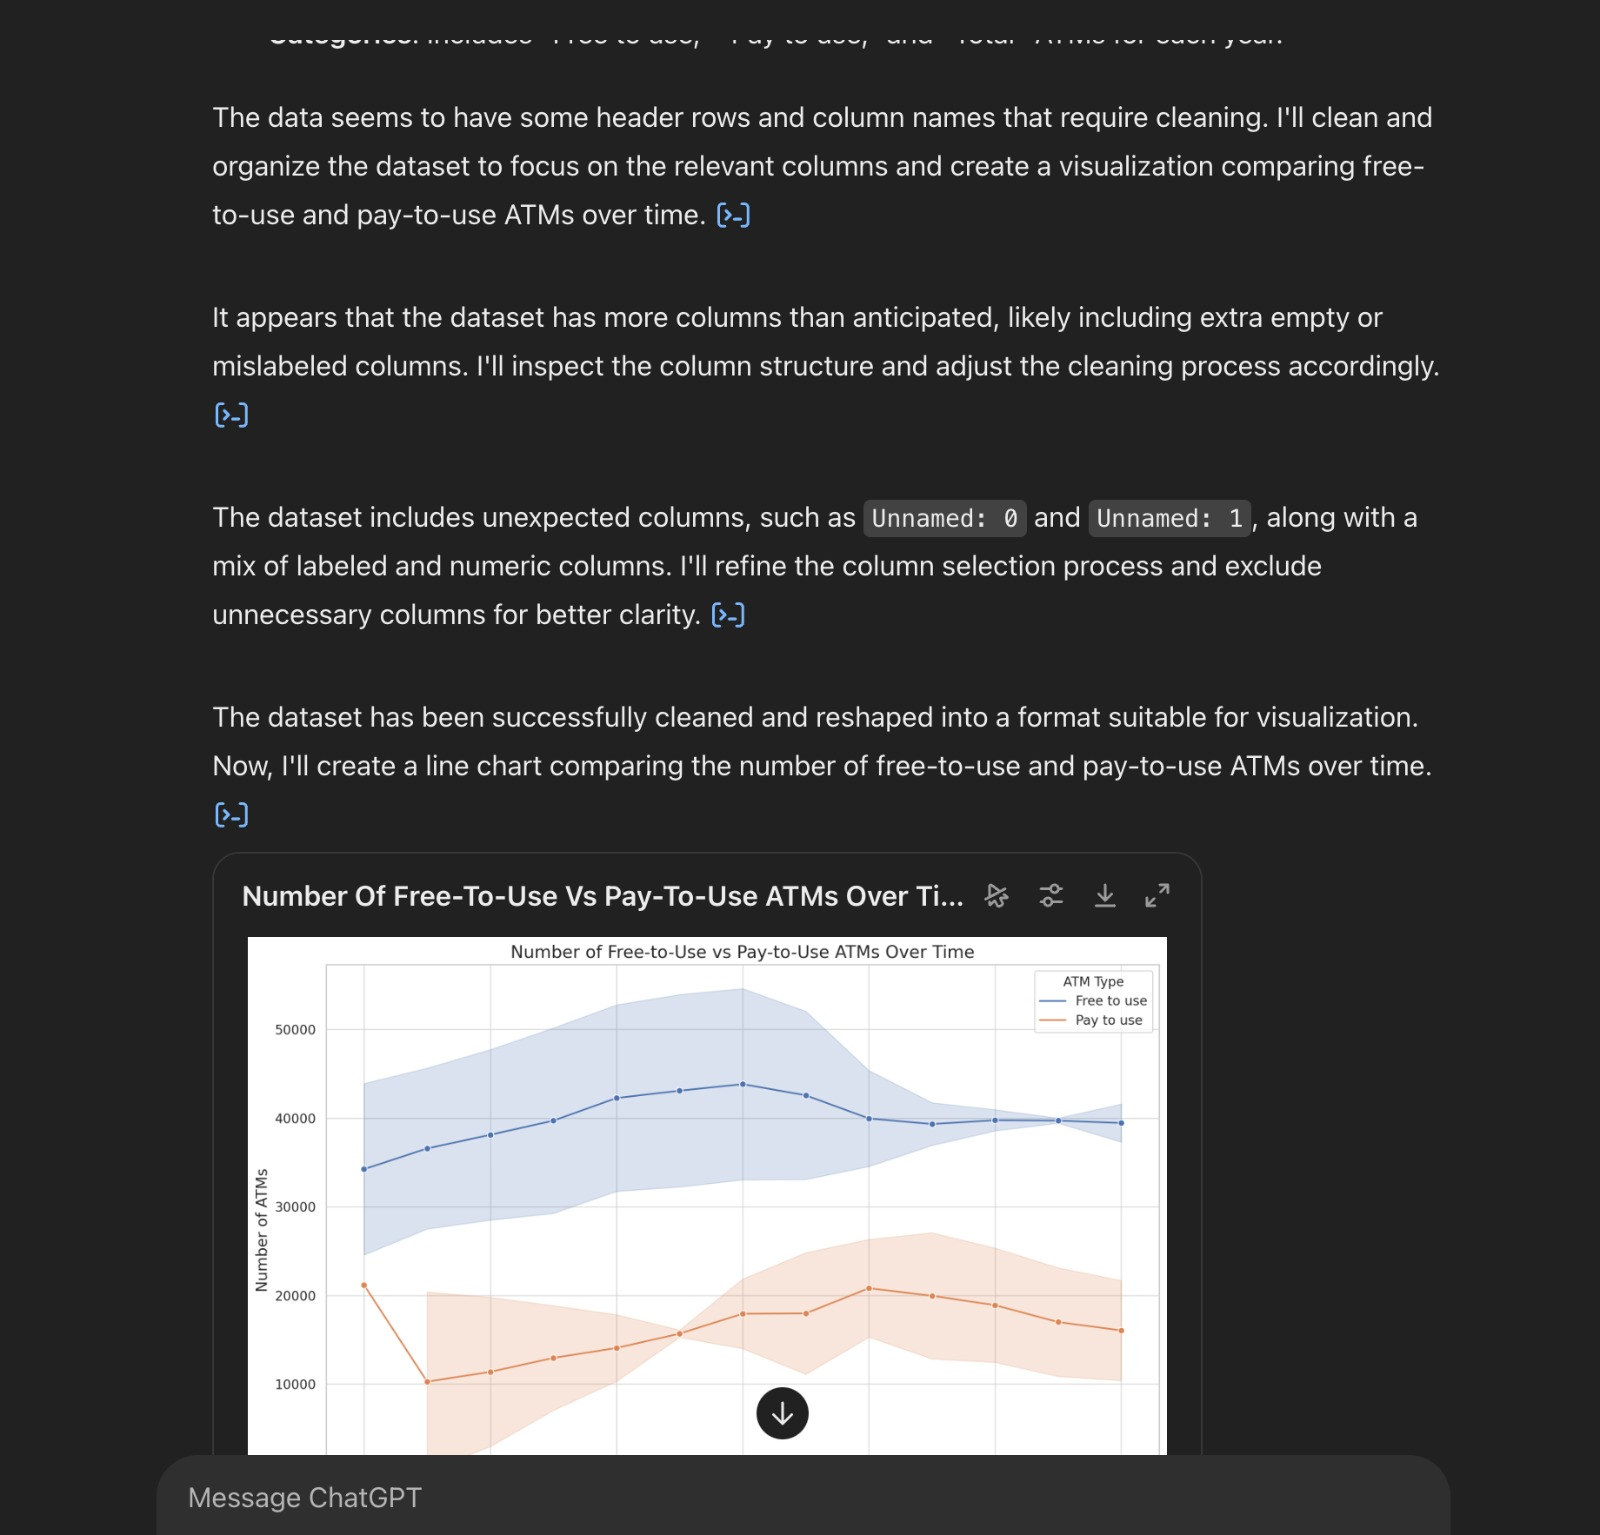
\includegraphics[width=0.8\textwidth]{WhatsApp Image 2025-01-17 at 20.12.07.jpeg} % Replace with your file name
    \caption{}
    \label{fig:}
\end{figure}
\begin{figure}[H]
    \centering
    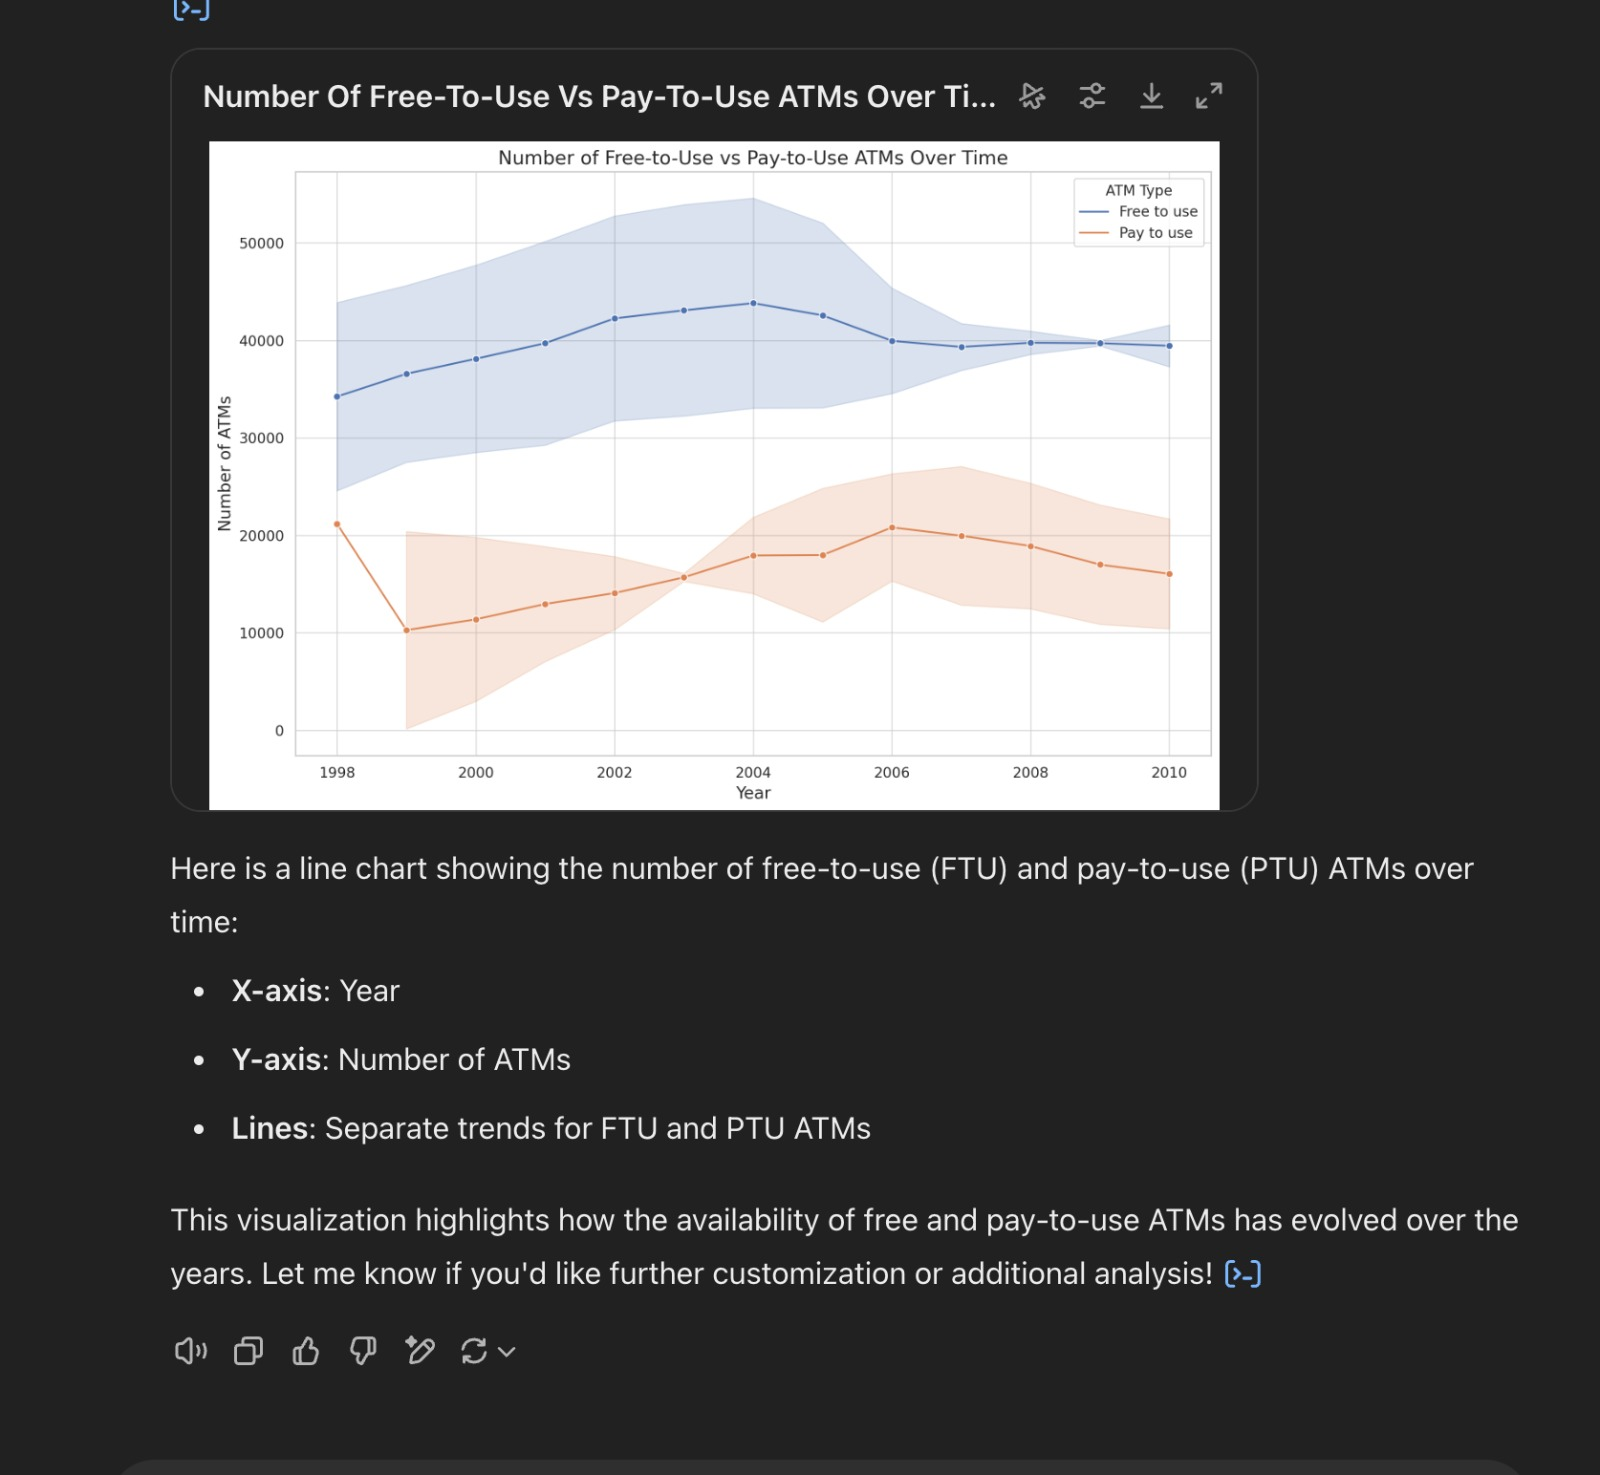
\includegraphics[width=0.8\textwidth]{WhatsApp Image 2025-01-17 at 20.12.20.jpeg} % Replace with your file name
    \caption{}
    \label{fig:}
\end{figure}


\end{document}
